\chapter{绪论}

\section{研究背景及意义}
近年来,喷水推进泵在高速船舶推进系统中得到了广泛应用,
随着动力传动系统与船体减振降噪技术的进步,推进泵噪声对舰船总体噪声的贡献度也被相对提高,
因而目前高新船舶对高效低噪声推进泵的需求日益迫切。
在满足推进性能需求的基础上,振动与声学特性目前已成为推进泵优化设计所关注的重点。
尤其在船舶推进领域,喷水推进泵水下噪声已经成为一项关键技术指标。

无论从推进泵低噪声设计或是从水声信号识别角度,对推进泵噪声的特性与机理开展研究均具有重要意义。
推进泵噪声机理较为复杂,抛开空化噪声不谈仅从流致噪声角度考虑,其频谱已呈现宽带与线谱交叠的形貌,
其中线谱噪声对噪声总级贡献度较大,很大程度上决定了推进泵的噪声水平。
前期研究发现,推进泵叶轮与其他部件之间的动静干涉是重要的线谱噪声激励源,
动静干涉的抑制因此成为降低推进泵线谱振动与噪声的有效方法之一。

牟介刚等人指 出无空化时泵喷负载噪声为主要噪声源
因此本文只对伴流场中泵喷推进器的负载噪声进行数值预 报"
 这同螺旋桨相似!无空化非均匀进流时!螺旋桨辐射噪声主要为桨叶非定常负载所致的流场压力 
 脉动产生的偶极子噪声

(1)从调制与解调的基本概念出发,采用基于循环平稳信号分析手段对推进泵噪声信号进行解调研究,
重点分析了推进泵的噪声调制特征机理,得到了在进速系数下的解调谱。
(2)基于labVIEW平台开发了推进泵振动噪声测试系统,开展了振动及噪声信号频率和特征、信号特征频段等研究,
为进行推进泵振动噪声测量、判断推进泵声学性能及进行噪声及流致激励源特性分析奠定了研究基础。 


\section{研究现状}
\subsection{推进泵噪声研究现状}
目前,国内外已经围绕螺旋桨、对转桨、推进泵等多种类型推进器的噪声开展了研究,
在噪声理论模型与噪声调制机理方面已有较多研究成果。
史广智[5]等人基于螺旋桨节拍对螺旋桨空化噪声的调幅作用,
研究了螺旋桨空化噪声理论模型与谐波族的关键特征。
曾赛[6]等人基于声学类比法建立了对转桨无空化噪声调制模型,研究了对转桨噪声的调制机理。
苏永生[7]等人分析了单级喷水推进泵空化噪声的调制特征,并研究了空化程度与噪声的关系。
总的来说,推进器伴流场谐调频率、叶片数与线谱噪声之间存在密切联系,
而循环平稳分析方法则是解调、量化这种联系的有效手段。

\subsection{循环平稳信号分析手段}
此外,离心泵工作环境一般比较复杂,因此其监测信号中多存在干扰。
因此,调制信号特征较弱,因此离心泵弱信号调制特征提取方法的研究尤为重要。
针对旋转机械监测信号特征提取的算法,国内外学者做了广泛的研究,
主要的信号解调方法有包络解调、谱峭度分析、循环平稳分析方法等。
在实际应用中包络解调应用最为广泛,现场的特征提取方式多采用该算法,
但是该方法的抗噪性能较差,弱信号的调制特征提取比较困难。
谱峭度分析方法是在包络解调算法的基础上发展而来,其更注重共振频带的识别,
对调制特征的提取依然为包络解调,因此该算法降低了解调谱中存在的干扰,
但是其弱信号的提取能力依然较差。循环平稳分析方法是一种高阶的特征提取算法,
该方法具有较好的抗噪性能,但是该算法的计算效率较低,
对于离心泵特征的在线监测与诊断应用比较困难,且解调谱中存在较多干扰频率特征。
因此,现有的弱信号特征的提取算法性能有待改进。

推进器、泵等旋转机械的噪声信号是周期性时变的,具有典型的循环平稳特征[8]。
其噪声信号常用的解调方法含包络分析、循环平稳分析等非平稳信号分析方法。
从解调调幅信号角度来看,在频率域上的包络谱分析方法等效于在循环频率域上的循环平稳分析方法,
但包络谱分析完全忽略了载波信息,无法揭示载波频率[9-10]。
而循环平稳自相关分析方法不仅具备包络谱分析的解调效果,可提取出调制特征信号,
同时具备功率谱密度分析方法的功效,可更好地支撑旋转机械噪声机理分析。
近年来,循环平稳分析方法开始用于机械故障检测以及旋转机械信号特征提取领域。
Antoni[11]较早研究了循环平稳分析方法在旋转机械噪声分析中的应用。
李诗佯[12]等人将CFD(计算流体力学)方法和循环平稳分析方法相结合,
建立了离心泵振动信号的幅值调制模型,研究了离心泵流致振动机理。
总的来说,对于信噪比低的旋转机械信号,例如处于复杂水声环境中的船舶推进器噪声,
循环平稳分析比包络谱分析具有更好的解调能力。

\section{研究内容和目标}
构建推进泵内流致激励源识别的有效方法和途径。
从噪声信号中分析出流致激励源的影响程度以及两者的作用机理

推进泵内由于非定常流动诱发的流致激励是推进泵噪声的根源,
噪声实则为流致激励的具体表现,
由于推进泵内部流动结构的多样性和复杂性,流致激励源信号也极为丰富,难
以直接对其展开研究,可以通过数值计算及试验手段精确提取相应信号。
因此,探寻合理、有效地信号处理与分析
方法,对于认清内流激励本质、揭示泵内流诱发振动激励机制至关重要。同时也
可为离心泵内非定常流动诱导振动机理的研究提供新方法,为泵的低振动噪声水
力设计提供参考。

推进泵噪声是推进泵流致激励特性的最直接的外在表现,构建流致激励与噪声之
间的关联对于推进泵低噪声设计及发展噪声能量主动控制技术至关重要。

非均匀流场与泵相互作用产生的非定常负载和压力脉动是推进泵流致激励的内在表现。


\subsection{研究内容}
\subsection{研究目标}

\chapter{推进泵噪声测试与分析系统设计}
\section{引言}
本研究基于LabVIEW平台开发了推进泵振动噪声测试系统,其中涵盖了信号采集的硬件系统设计,
以及实现信号分析和存储的软件系统设计,该系统支持同步对多通道传感器信号实时采集,各通道信号同时处理、显示及存储,
同时也能够实现振动加速度传感器的性能检验和指标评估,不仅适用于推进泵振动及噪声测试场景,
也可以推广到离心泵、风机等动设备振动与噪声测试场景中使用。

基于此平台可开展对振动及噪声信号频率和特性、特征频段等研究,
为进行推进泵振动噪声测量、判断推进泵声学性能及进行噪声及流致激励源特性分析奠定了研究基础。

\section{系统总体设计概述}
\subsection{推进泵试验台简介}
本研究依托上海船舶运输研究所(SSSRI)的空泡水洞,针对推进泵样机模型开展了噪声性能的试验研究。
空泡水洞由德国KEMPF\&REMMERS公司制造,如\autoref{fig:tube1}和\autoref{fig:tube2}所示。
水洞整体采用不锈钢材料,配有压力调节箱和除气装置,具有很好的可控性。
水洞工作段长2.6m,横截面呈方形带圆角,尺寸为0.6m×0.6m。
\begin{figure}[htbp]
    \centering
    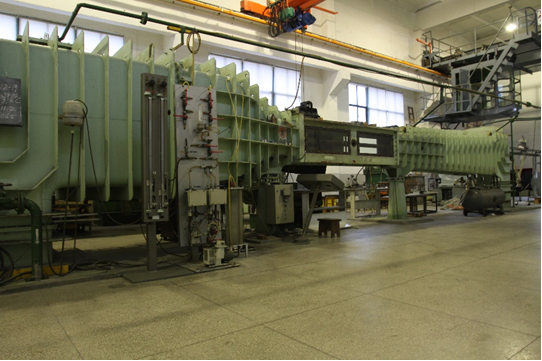
\includegraphics[scale=0.75]{3水洞1.png}
    \caption{\label{fig:tube1}SSSRI空泡水洞}
\end{figure}
\begin{figure}[htbp]
    \centering
    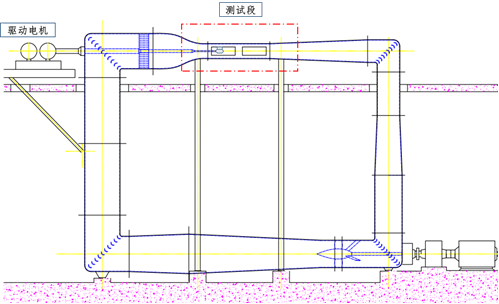
\includegraphics[scale=0.85]{3水洞2.png}
    \caption{\label{fig:tube2}水洞整体结构}
\end{figure}

水洞工作段如\autoref{fig:work}所示,最高水速可达12m/s。
缩比模型样机悬挂于水洞上壁面,导管由光折射率与水一致的透明有机玻璃制成,以确保其内流场的可视性。
水筒侧面有机玻璃外安装一小型水舱,将水听器置于其中,测量推进泵在多工况下运转的水下噪声。
\begin{figure}[htbp]
    \centering
    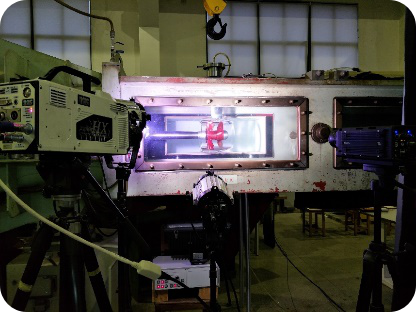
\includegraphics[scale=1.2]{3水洞工作段.png}
    \caption{\label{fig:work}水洞工作段}
\end{figure}

水洞的水动力测试系统采用安装在传动轴上的动力仪测量叶轮和导流锥上产生的推力和转矩,
动力仪测量的最大推力为3000N,最大扭矩为150N$\cdot$m,测量精度0.2\%,最大转速4000rpm,能满足推进泵模型的测试需求。
采用五分量测力天平测量导管和导叶等静止部件的受力情况。
水洞内的水速、压力信号和动叶的推力、扭矩和天平信号经放大器放大后送计算机进行A/D转换并处理,转速信号通过频率计同步输入计算机。

为了分析推进泵在不同水动力性能下的噪声特性,对推进泵的水动力特性和水动力噪声同时进行了测量。
推进泵噪声测试系统的示意图如\autoref{fig:equipment}所示,主要包括测试推进泵、水洞、水听器、
数据采集卡、电脑(上位机软件)五部分组成。
\begin{figure}[htbp]
    \centering
    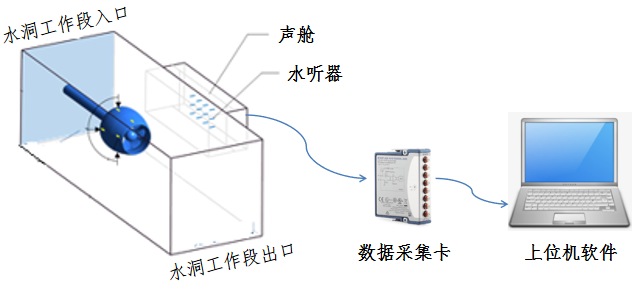
\includegraphics[scale=0.75]{3测试系统.png}
    \caption{\label{fig:equipment}推进泵噪声测试系统装置示意图}
\end{figure}

\subsection{测试基本参数和数据处理}
本研究设计的测试信号对象包括声压和振动加速度信号,用来表征测试对象的声学和振动性能,可分别由麦克风或者水听器和
振动加速度传感器测量。信号处理主要涉及频谱分析和1/3倍频程分析。

在振动与噪声信号的分析中,声压级和振动加速度级是常用的参数,一个声学量的级是该量与同类量的基准值之比的对数。
其中,声压级定义为将待测声压$p_e$与参考声压$p_{ref}$的比值取常用对数,再乘以20,以分贝计,即
\begin{equation}
    \label{equ:p}
    L_{p} = 20\log_{10}{\left(p_{re}/p_{ref}\right )}
\end{equation}
式中,在水中基准声压为$p_{ref}= 1\times 10^{-6} \mathrm{P} a$,在空气中基准声压为$p_{ref}= 2\times 10^{-5} \mathrm{P} a$。
同理,振动加速度级也定义为加速度有效值$a_e$与基准加速度$a_{ref}$之比的以10为底的对数,再乘以20,以分贝计,即
\begin{equation}
    \label{equ:a}
    L_{a} = 20\log_{10}{\left(a_{re}/a_{ref}\right )}
\end{equation}
式中,基准加速度值为$a_{ref}= 1\times 10^{-6} \mathrm{m/s^2} $。

信号的频谱是指信号的频率成分与能量分布的关系,可以体现信号的频率特征。在振动与噪声信号的分析中,
通常也会采用1/3倍频程频谱分析,是比较符合人耳分辨频率能力的频带划分方法,能更加详细的反映噪声源的频谱特性。
通过将整个频谱划分为若干频带,每个频带的上限频率$f_u$与下限频率$f_l$之比是2的立方根,即满足以下公式:
\begin{equation}
    \label{equ:fu}
    f_{u}/f_{l}=2^{1/3}=1.2599
\end{equation}
中心频率f$_{m}$为上下限频率的几何平均值,即
\begin{equation}
    \label{equ:fm}
    f_{m}=\sqrt{f_{u}\cdot f_{l} } 
\end{equation}
本研究进行1/3倍频程分析所采用的方法是通过对采样信号进行快速傅立叶变换,计算出功率谱或幅值谱,
然后用功率谱或幅值谱的数据,计算每一个中心频率带宽的信号有效值,代入\autoref{equ:p}或\autoref{equ:a}
中可得到该频段内的声压级。
\subsection{测试系统基本方案}
本研究所采用的技术框架如\autoref{fig:framework}所示,主要包括传感器,信号调理模块,数据采集卡和上位机分析软件。
\begin{figure}[htbp]
    \centering
    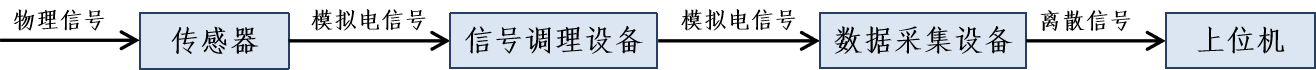
\includegraphics[scale=0.55]{2硬件设备流程图.png}
    \caption{\label{fig:framework}技术框架图}
\end{figure}

目前国内在数据采集卡和上位机分析软件的结合方面主要采用的方式有两种,
一种是购买国内公司的数据采集卡,然后自行设计上位机分析软件,这种方案价格低廉,
但是自行开发上位机软件周期长,且功能有限还不易扩展。
另一种是购买美国NI公司的LabVIEW软件和数据采集卡套件,NI公司的虚拟仪器系统灵活性高,
开发成本更低,同时数据采集卡套件系统具有更小尺寸,但是价格非常高昂。
针对本研究所涉及的泵或风机等测试场景,选用开发灵活性更高且尺寸更小的硬件系统更为合适,
因此本研究采用的是美国NI公司的LabVIEW软件和数据采集卡套件。

通过LabVIEW调用硬件设备的底层驱动程序,结合软件功能模块,从而搭建出控制数据采集传输,处理和存储的系统。
该系统的的核心部分是功能模块的设计,本系统功能模块可分为系统设置模块、信号采集模块、数据显示模块、信号分析模块、数据管理模块等,
系统方案图如\autoref{fig:system}所示。此外还可以根据实际情况,灵活地添加新的功能模块。
在2.3节软件系统设计中将对软件模块的设计过程作详细介绍。
\begin{figure}[htbp]
    \centering
    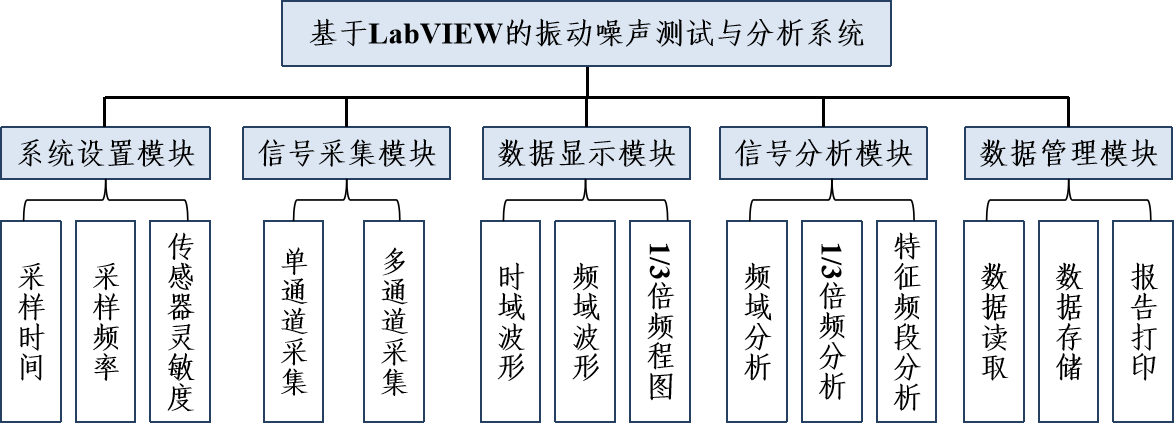
\includegraphics[scale=0.6]{2系统方案.png}
    \caption{\label{fig:system}系统方案图}
\end{figure}

\section{测试系统硬件设计}
针对本研究所涉及的泵或风机等测试场景,传感器需要支持远距离传输,简单电路调理等功能,
因此本研究选用了抗干扰能力强,内置放大器等要求的传感器类型。
传感器由于内置了专门的集成调理电路,属于有源传感器,而该电路要正常工作需要恒流源供电。
这样一来,一方面系统可以不用设置额外的信号调理设备,简化了测试系统。
另一方面对数据采集设备也提出了要求,主要包括以下几个方面,(1)支持多通道同步采集;
(2)支持IEPE信号调理;(3)轻巧灵活,便携式;(4)支持USB外设总线技术。

综合考虑以上因素,本研究选用了​NI9234采集卡,如\autoref{fig:acquire}所示。
​NI9234是美国NI公司的一种4通道高速动态信号采集卡,兼容USB接口,AC/DC耦合方式可选,
可对IEPE传感器进行高精度测量。
NI9234带有2mA恒定电流的集成电路压电式(IEPE)信号调理,包含内置抗混叠滤波器,
可自动调节至设置的采样率,也对采集系统进行了接地屏蔽处理,
输入通道可同时以最高为51.2$\mathrm{kHz}$的速率对信号进行数字化。
\begin{figure}[htbp]
    \centering
    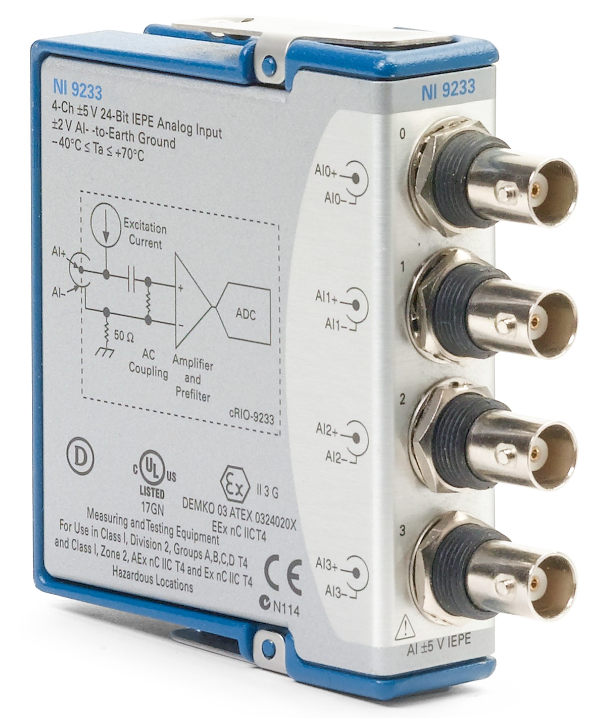
\includegraphics[scale=0.3]{2数据采集卡.png}
    \caption{\label{fig:acquire}数据采集卡}
\end{figure}
​
数据采集卡每个通道的输入信号经缓冲,放大器和预滤波器调理后,由模数转换器对其采样。

数据采集卡系统结构如\autoref{fig:acquire}所示。
数据采集卡采集数据时,数据传输方式包括直接内存访问(DMA),中断请求(IRQ)和可编程I/O。
DMA是一种DAQ板卡和PC内存间直接通讯的传输方式,不再需要处理器的干预。
NI "MITE"芯片可以处理与PCI总线间的所有总线协议。
IRQ传输方式会置高信号并中断处理器,然后由处理器处理数据传输。
IRQ  传输通常很低,只有150 kb/s,而DMA可以高达20 Mb/s。
IRQ 传输速率与使用的系统设备相关,如处理器速度等。
NI数据采集系统中默认是使用DMA传输方式。

数据采集卡的传输过程为,外部的信号进入数据采集卡后,经过各种处理转换,
先进入数据采集卡自身的缓冲区里面,缓冲区是先进先出(FIFO,First In First Out)的。
NI的数据采集卡有板载的缓冲区,不同数据采集卡的缓冲区的大小不一样,
板载缓冲区的大小一般是出厂商固定的,无法更改。
然后当板载缓冲区中的数据量到了一定的条件时,数据采集卡将缓冲区的数据上传到计算机内存中,
一般是以DMA(直接内存访问)方式传入的。

\begin{figure}[htbp]
    \centering
    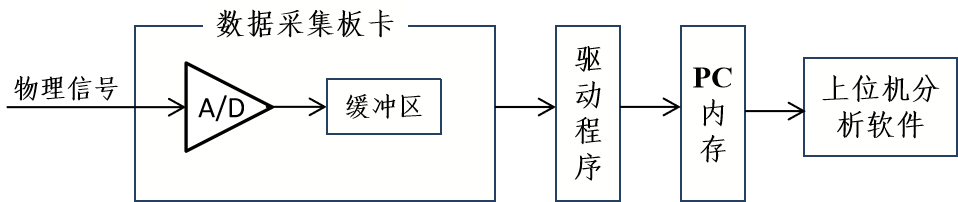
\includegraphics[scale=0.6]{2数据采集卡系统结构.png}
    \caption{\label{fig:acquire}数据采集卡系统结构}
\end{figure}

\section{测试系统软件设计}
在对软件系统进行设计之前,最先需要考虑的是计算机与硬件的交互。
和硬件交互需要两个基本要素:第一,硬件和计算机的通信接口和通信协议。
常用的接口及协议有USB 、LAN和PXI通信总线等等;
第二,交互命令,即通过上述通信接口按照协议发送的逻辑程控指令,例如仪器程控中常见的有VISA 、SCPI命令架构体系。

LabVIEW最大优势就是和测量硬件交互的便利性。
因为一方面NI公司将与硬件交互的逻辑指令按功能组织成硬件驱动(driver),可以直接下载安装。
另一方面NI的数据采集板卡一般都支持多种外设总线技术,比如PCI、USB,
外设总线的作用是允许外部IO设备与计算机CPU和内存通信。
使用LabVIEW连接硬件系统往往需要一个工具软件NI的MAX,即Measurement\&Automation Explorer(MAX),
用来验证驱动安装与否和连接的正常性检查。
在我们安装好驱动之后,用NI MAX软件验证连接和驱动的工作正常性,
之后就可以开始在LabVIEW中进行编程来实现具体的业务功能。

LabVIEW是图形化的编程语言,编程方法不同于传统程序设计方法, 它摆脱了传统语言线性结构的困扰, 
执行顺序是由数据流的方式确定。
本研究基于LabVIEW面向过程的编程思想,使用了通知器、队列和事件的设计模式,
实现了系统设置模块、信号采集模块、数据显示模块、信号分析模块、数据管理模块等模块的设计。
软件的主界面如\autoref{fig:main}所示,各功能模块集成到该主界面上。
\begin{figure}[htbp]
    \centering
    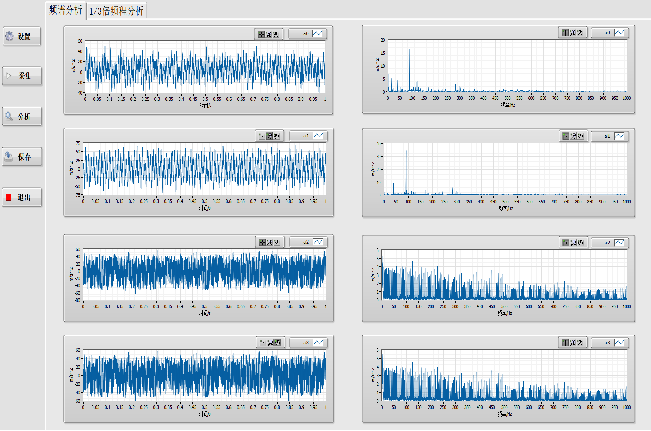
\includegraphics[scale=0.25]{2软件主界面.png}
    \caption{\label{fig:main}软件主界面}
\end{figure}

推进泵噪声测试系统测量流程是:首先等待各部分参数设置好后,发出采集启动信号,
同步采集各通道数据,采集完成后数据自动存储在相应文件中。信号分析会从文件中读取数据,
分析结果实时展示在界面。程序设计流程如\autoref{fig:process}所示。
\begin{figure}[htbp]
    \centering
    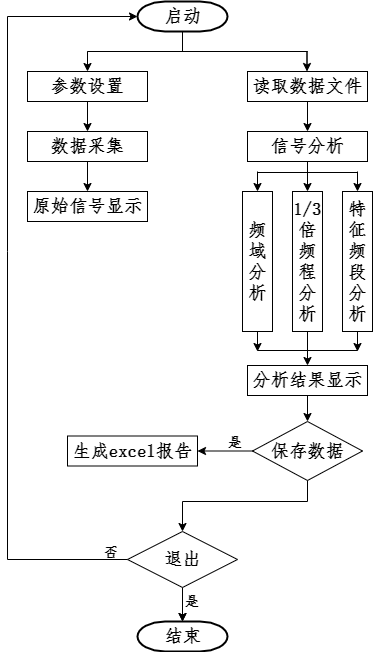
\includegraphics[scale=0.55]{2软件流程图.png}
    \caption{\label{fig:process}程序流程图}
\end{figure}

\begin{comment}
\subsection{系统设置模块}
软件界面的设置模块提供了测试系统各项参数设定,包括采集通道设置、采样参数设置、
传感器灵敏度设置、分析参数设置等。
\begin{figure}[htbp]
    \centering
    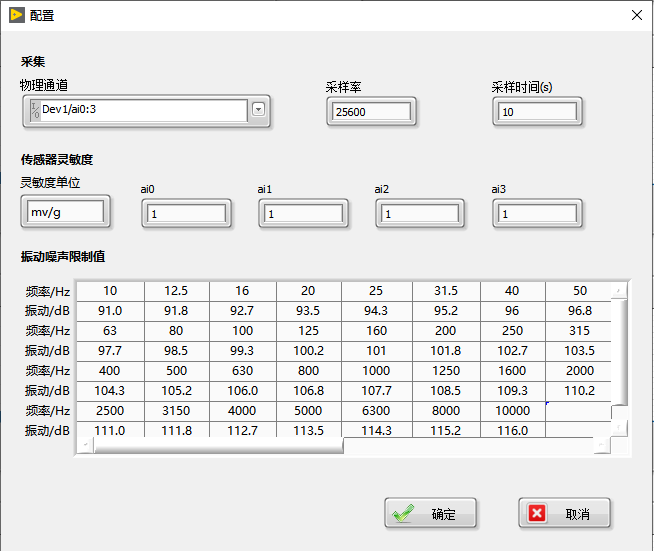
\includegraphics[scale=0.55]{2系统设置.png}
    \caption{\label{fig:setting}系统设置}
\end{figure}
\end{comment}

\subsection{数据采集模块}
在对数据采集模块进行设计时,本研究主要考虑如下几个方面:(1)如何保证数据在采集过程中不丢失?
(2)实现采集数据的实时存储。
在2.2节提到程序最终是从计算机内存读取数据,而这个缓存区的大小是我们可以指定的。
缓冲区存储数据量的大小又是和它的输入速度和输出速度有关,输入速率是由采样率所决定的,
输出速度就是采集程序从它里面读取的速度。
假如计算机内存缓冲区设置的过小,或者输出速率过慢,都有可能导致缓存区的溢出,出现数据丢失的情况。
计算机内存缓冲区设置的过大,在硬盘和内存之间会产生过量的读写操作,也会对系统性能造成影响。
所以为了保证数据不会丢失,要设置好内存缓冲区的大小,
还要保证读取缓冲区的程序(DAQmx Read.vi)循环得尽量快,每一次读取的数据尽量多。
LabVIEW中缓冲区大小的设置也和采样模式有关,常用的采样模式为有限采样和连续采样,本研究采用连续采样模式。
对于连续采样模式,NI-DAQmx设置的缓存区大小如\autoref{tab:sample}所示,缓存区大小建议是采样率的10倍左右。
对于读取缓冲区的程序(DAQmx Read.vi)来说,设置成多采样,每次都是将内存中的所有数据读取进来,就能实现读取的数据尽量多。
\begin{table}[htbp]
    \centering
    \caption{\label{tab:sample}NI-DAQmx连续采样缓存区大小}
    \begin{tabular}{ccc}
     \toprule
     采样率&缓冲区大小\\
     \midrule
     未指定速率&10 kS\\
     0-100 S/s&1 kS\\
     100-10,000 S/s&10 kS\\
     10,000-1,000,000 S/s&100 kS\\
     >1,000,000 S/s&1 MS\\
     \bottomrule
    \end{tabular}
\end{table}

为实现数据的实时存储,本研究采用了生产者/消费者的模式,
生产者/消费者结构基于队列的数据结构,即开辟一个缓存区,依据先进先出的原则进行。
新来的元素总是被加入队尾,每次离开的元素总是从队首离开。程序中新采集的数据加入到
队尾,队首出队的元素同步保存在相应文件中。
这样就保证了数据存储过程中不会出现数据丢失的现象,能实现实时存储。
数据采集程序框图如\autoref{fig:soft}所示。
\begin{figure}[htbp]
    \centering
    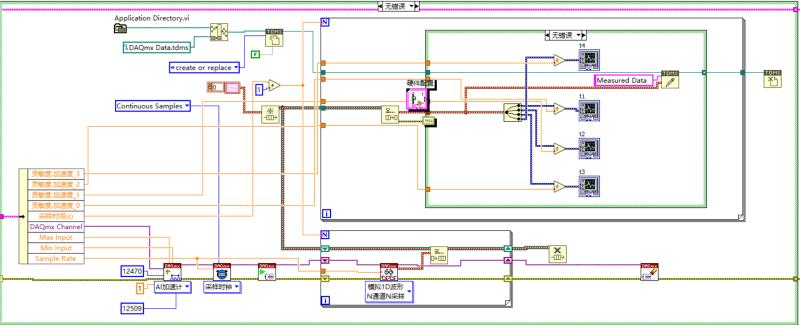
\includegraphics[scale=0.85]{2数据采集程序框图.jpg}
    \caption{\label{fig:soft}数据采集程序框图}
\end{figure}


\subsection{信号分析模块}
LabVIEW以G编程语言为基础,尤其适合于数据采集、仪器控制、和图像显示等应用,可以高效地构建虚拟仪器系统。
然而这种图形化的软件开发环境对于复杂的数值计算和分析要求就显得力不从心,
在对各种信号分析算法的支持方面,LabVIEW的工具箱也非常有限。
LabVIEW8.2以后版本推出了仿真框图和面向数学的文本编辑语言MathScript,它带
有交互式窗口和可编辑的接口,通过MathScript用户可以在LabVIEW图形化程序中运行较简单的m文件语法脚本。
因此LabVIEW提供了与MATLAB进行通信的方式,本研究借助数据处理能力更强的MATLAB进行信号的分析。

MATLAB也支持ActiveX自动化技术,LabVIEW程序在运行MATLAB Script节点时,会启动一个MATLAB进程执行脚本的内容,
并且与MATLAB的工作空间进行数据交换。但是MATLAB Script节点对输入、输出数据的类型有明确的要求,只有
LabVIEW中的数据类型与MATLAB中的数据类型相匹配,才能够进行数据交换。
将采集模块中获取的数据导入如\autoref{fig:otc}所示的节点中,便可对信号进行频谱分析和1/3倍频程分析,
软件分析模块的界面如\autoref{fig:analyze}所示。
\begin{figure}[htbp]
    \centering
    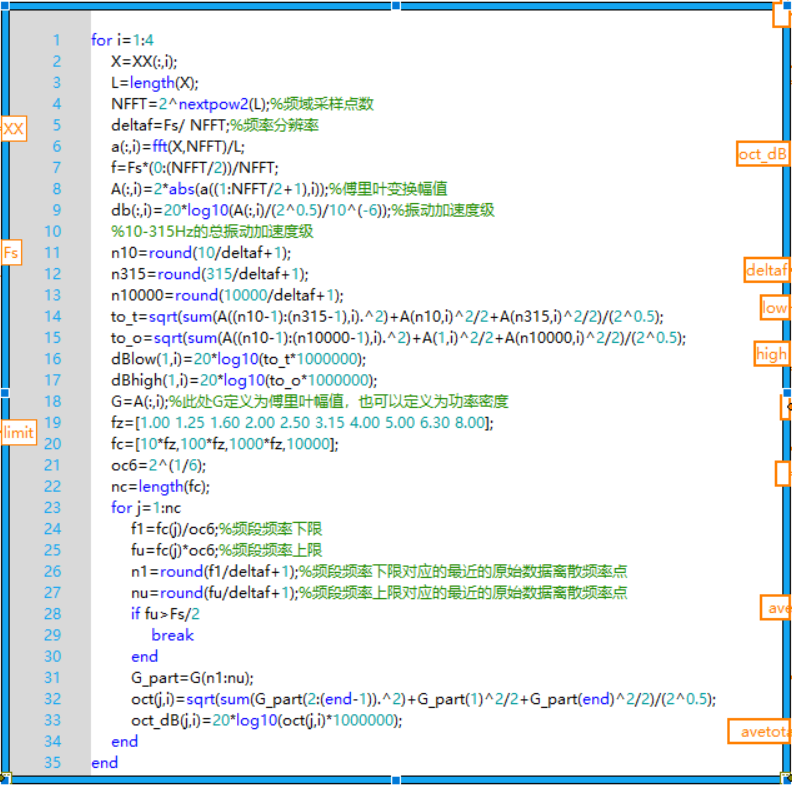
\includegraphics[scale=0.75]{2倍频程程序.png}
    \caption{\label{fig:otc}mathscript节点部分进行1/3倍频程分析的程序}
\end{figure}

\begin{figure}[htbp]
    \centering
    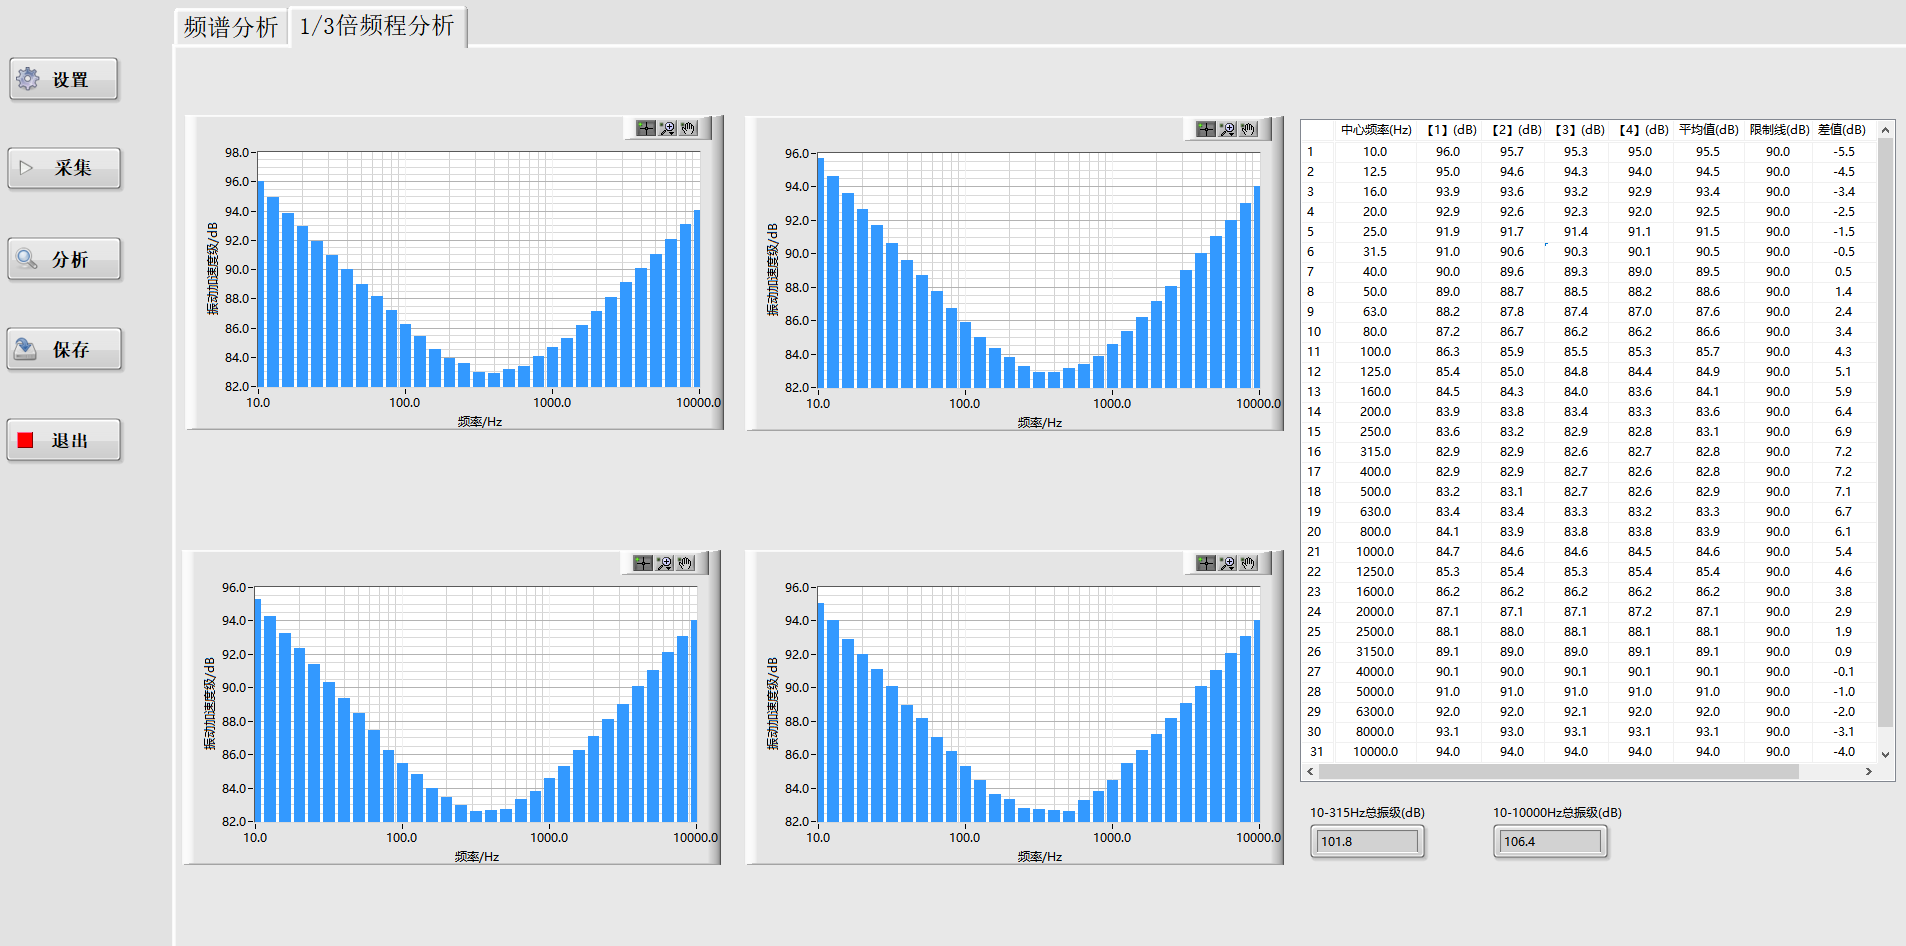
\includegraphics[scale=0.25]{2软件分析模块.png}
    \caption{\label{fig:analyze}mathscript节点部分进行1/3倍频程分析的程序}
\end{figure}

\subsection{数据管理模块}
数据管理模块包含采集数据的实时存储、采集数据的读取和分析数据的存储。
由于实验是多通道数据采集,且采样速度要求较高,因此数据量较大。为了方便实时存储和
管理这些数据,程序采用TDMS文件格式。TDMS文件格式是NI主推的一种二进制记录文件,
它兼顾了高速、易存取和方便等多种优势,在记录的仿真或测量数据的同时,也会存储描述性信息,
包括测试过程,传感器信息等,数据实时存储程序框图如\autoref{fig:save}所示。当数据采集完成进行分析时,程序会从已保存的TDMS文件中读取数据
导入分析模块进行,数据读取程序框图如\autoref{fig:read}所示。分析完成数据将会以excel表格的形式进行存储。
主程序中从VISAread的readbuffer端读上来的数据需要转换成表格数据进行保存,
数据的保存分为两个阶段。第一阶段,通过表单形式(带时间头)显示在主程序界面,
方便用户直观查看测试参数是否已满足要求。
第二阶段,把表单数据保存到Excel文件中,可供用户打印查询。
\begin{figure}[htbp]
    \centering
    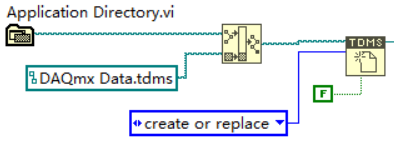
\includegraphics[scale=0.85]{2文件存储.png}
    \caption{\label{fig:save}数据实时存储程序框图}
\end{figure}
\begin{figure}[htbp]
    \centering
    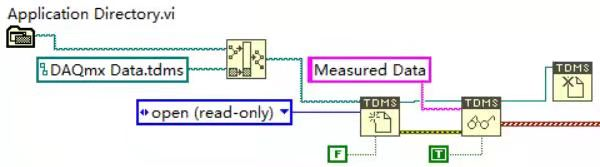
\includegraphics[scale=0.45]{2文件读取.jpg}
    \caption{\label{fig:read}数据读取程序框图}
\end{figure}
%\section{性能测试}
\section{本章小结}
本章针对推进泵噪声试验平台振动噪声测试系统中的硬件系统设计和软件系统设计,
采用美国pcb手持式校准器394C06进行校准。

\chapter{推进泵噪声特性的试验研究}\label{ch:chapter3}
\section{引言}
本文以紧凑型前置导叶的单级推进泵和新型结构的双级推进泵这两种型式的推进泵为研究对象,
在大型空泡水洞中对其进行噪声试验研究,
试验中通过固定叶轮转速、改变水洞流速的方法,从而获得推进泵在不同水动力性能工况下的噪声数据。
由于水听器所处的非消声环境会影响推进泵中低频段辐射噪声的可信度,本研究对多工况下的水洞背景噪声
进行了试验测量,分析了水洞背景噪声的频谱特性和特征频段能量分布,试图剥离背
景噪声对推进泵噪声的干扰。
最后,基于噪声采集与分析系统的分析模块,借助频谱分析和三分之一倍频程分析等信号分析手段对推进泵噪声数据进行处理,
探讨推进泵噪声特性,阐明水速对推进泵噪声各频段的影响,以及各频段噪声对
推进泵噪声总声压级的贡献度。
\section{单级推进泵噪声特性的试验研究}
\subsection{推进泵试验模型}
本小节的研究对象是一种紧凑型前置导叶推进泵,
设计参数根据某航行体的推进需求计算,并进行缩尺得到。
最终确定轮缘直径200mm,并采用11片导叶加7片叶片的形式。
导管的设计选用33号减速喷管,可在一定程度上降低入流速度充分提升叶轮的抗空化性能,
并根据动量定理确定导管得出口直径,保证推进器能产生足够的推力。
导叶设计的核心问题就是如何设置合理的预旋,来达到更高的效率,
导叶的作用方式如\autoref{fig:daoye}所示。
\begin{figure}[htbp]
    \centering
    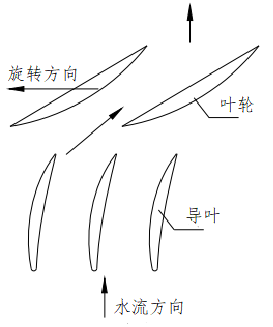
\includegraphics[scale=1.0]{3导叶作用方式.png}
    \caption{\label{fig:daoye}导叶作用方式}
\end{figure}
叶轮的设计主要考虑了以下几个方面:(1)将定转子间距增大为0.2倍轮缘直径来减小定转子之间干涉;
(2)通过缩短叶顶长度进一步减小叶轮顶部的载荷,来减小叶顶泄漏带来的效率损失,提升推进器总体能效水平;
(3)将叶轮剖面翼型的最大厚度后移到40\%弦长处,优化吸力面压力分布,延迟空化的发生。
推进泵设计模型如\autoref{fig:dj_design}所示。
\begin{figure}[htbp]
    \centering
    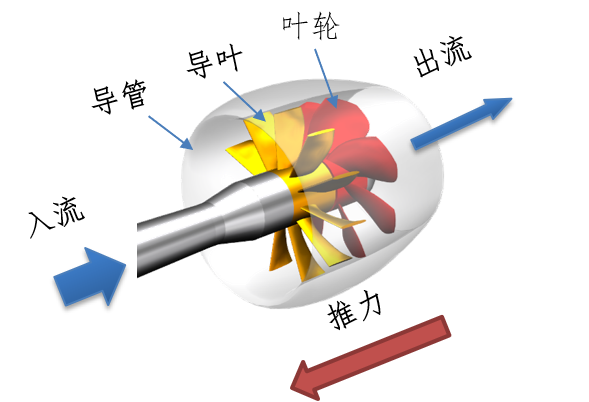
\includegraphics[scale=1.0]{3单级整体结构.png}
    \caption{\label{fig:dj_design}单级推进泵设计模型}
\end{figure}

推进泵的设计参数如\autoref{tab:dj}所示。
\begin{table}[htbp]
    \centering
    \caption{\label{tab:dj}单级推进泵设计参数}
    \begin{tabular}{ccc}
     \toprule
     参数&值\\
     \midrule
     D(叶轮直径,mm)&200\\
     N(设计转速,rpm)&1260\\
     L(导管长度,mm)&240\\
     $D_1$(入口直径,mm)&228\\
     $D_2$(出口直径,mm)&182\\
     $Z_1$(叶轮叶片数)&7\\
     $Z_2$(导叶叶片数)&11\\
     轮毂比&0.3\\
     旋向&右旋\\
     \bottomrule
    \end{tabular}
\end{table}
推进泵试验模型的叶轮采用铝合金加工制造,表面做阳极化处理。导管选用有机玻璃材质,便于观察其特性。
单级推进泵试验模型如\autoref{fig:dj_test}所示。
\begin{figure}[htbp]
    \centering
    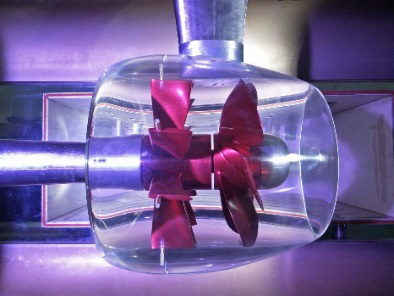
\includegraphics[scale=2]{3单级试验模型.png}
    \caption{\label{fig:dj_test}单级推进泵试验模型}
\end{figure}
为了获得推进泵在不同水动力工况下的噪声数据,
试验中通过固定叶轮转速、改变水洞流速的方法测量了不同进速系数工况点下的
水动力性能和噪声数据。

在推进泵水动力性能试验方面,结合主轴扭矩与转速等数据计算推进泵叶轮的功率、扬程、水力效率,
借助动力仪测量多工况下泵喷推进器的推力性能,可得到推进器的敞水性能曲线。
空泡水筒测力系统可以独立测量旋转部件和静止部件产生的推力,
由天平测量得到导管和导叶(包括连接机翼阻力)的总推力$T_{D}$。
导管和导叶推力为天平测得的总推力减去导管连接机翼阻力$(F)$,
即$T_{D}=T_{D}-F$。在均匀流场常压条件下,推进器模型敞水性能试验采用定转速,
改变来流速度以获得相应于各个进速系数$J$的推力系数,扭矩系数$K_{Q}$等水动力数据。
推力系数、扭矩系数等定义如\autoref{equ:three1}-\autoref{equ:three7}所示。
\begin{equation}
    \label{equ:three1}
    J=\frac{V}{nD} 
\end{equation}
\begin{equation}
    \label{equ:three2}
    Re =\frac{C_{0.7R}\sqrt{V^{2}+\left ( 0.7\pi nD \right )^{2}   }  }{\upsilon } 
\end{equation}
\begin{equation}
    \label{equ:three3}
    K_{T}=\frac{T}{\rho n^{2}D^{4}  }  
\end{equation}
\begin{equation}
    \label{equ:three4}
    K_{TP}=\frac{T_{P} }{\rho n^{2}D^{4}  }  
\end{equation}
\begin{equation}
    \label{equ:three5}
    K_{TD}=\frac{T_{D} }{\rho n^{2}D^{4}  }  
\end{equation}
\begin{equation}
    \label{equ:three6}
    K_{Q}=\frac{Q}{\rho n^{2}D^{4}  }  
\end{equation}
\begin{equation}
    \label{equ:three7}
    \eta _{0} =\frac{J}{2\pi } \cdot \frac{K_{T} }{K_{Q}} 
\end{equation}

式中$D$表示叶轮直径$(m)$,$V$表示来流速度$(m/s)$,$n$表示转速$(r/s)$,
$Re$表示雷诺数,$C_{0.7}$表示叶轮0.7R处的弦长$(m)$,
$T$表示推进泵总推力$(N)$,$T_{P}$表示动叶推力$(N)$,
$T_{D} $表示导管加支架推力$(N)$,
$F$表示导管测力连接机翼阻力$(N)$,
$Q$表示扭矩$(N \cdot m)$,$K_{T}$表示推力系数,$K_{TP}$表示动叶推力系数,
$K_{TD}$表示导管支架推力系数,$K_{Q}$表示扭矩系数,
$\eta _{0}$表示效率。

将水洞试验测得的单级推进泵推力、转矩和效率等数据无量纲化后,得到如\autoref{fig:chanshuiquxian}所
示的敞水性能曲线。从图中可以看出:随着进速系数J的增大,
推力系数$K_T$和转矩系数$K_Q$逐渐减小,而推进效率$\eta_0$先增大后减小,
并在 J=1.0 处有最大值 61.2\%。与常见的螺旋桨敞水性能
曲线相比,单级推进泵的敞水性能曲线随进速系数增加时变化趋势平缓,具有较高推进
效率的同时也有较宽的高效工作区。
\begin{figure}[htbp]
    \centering
    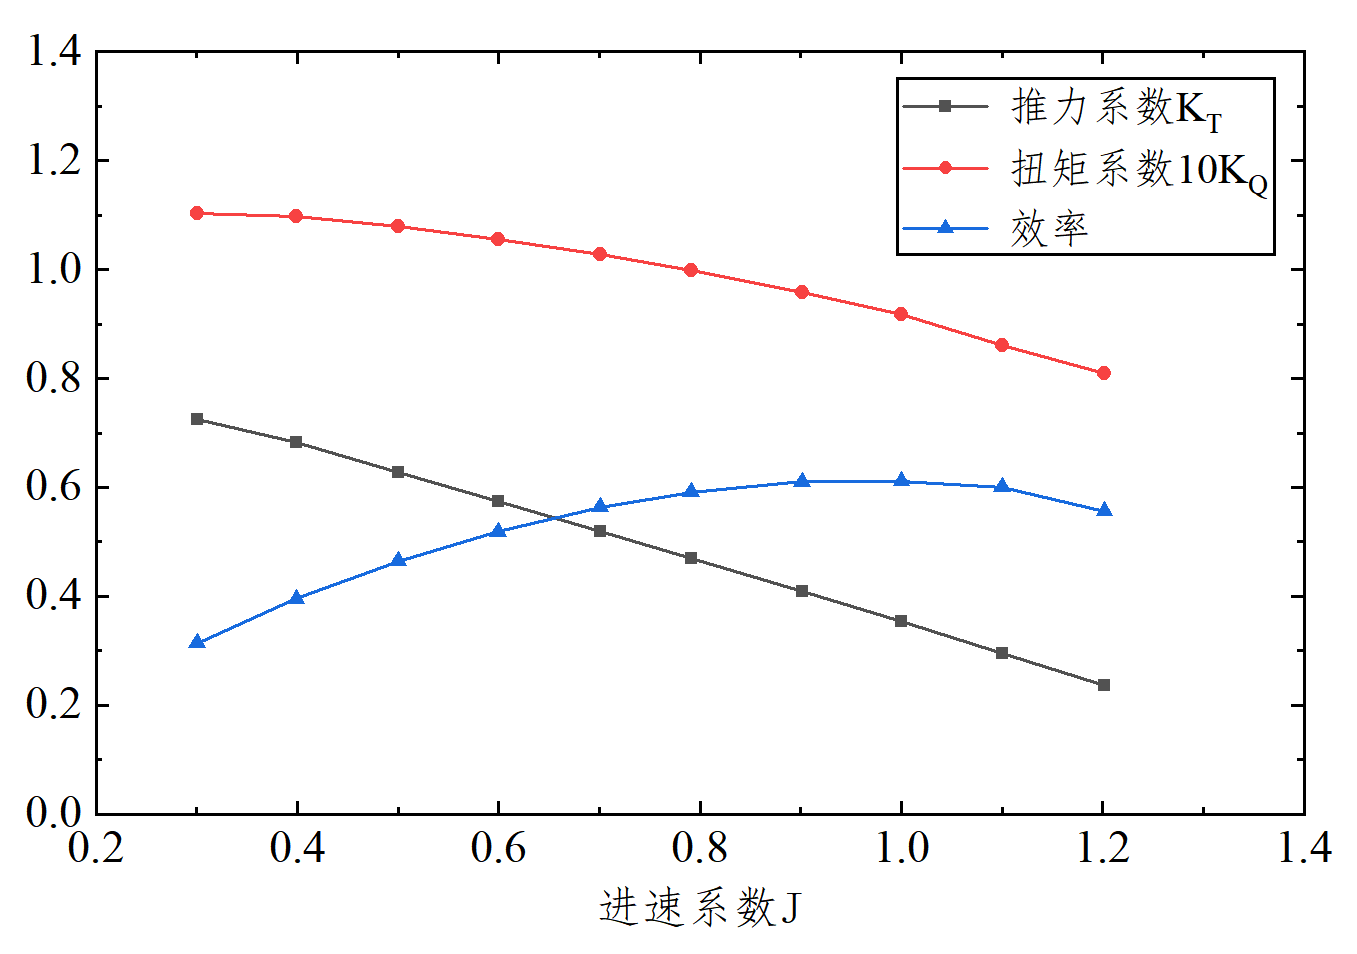
\includegraphics[scale=1]{3单级性能试验.png}
    \caption{\label{fig:chanshuiquxian}单级推进泵敞水性能曲线}
\end{figure}

在噪声试验方面,采用水听器作为声学传感器。
由于推进泵声信号覆盖了从几百到几千赫兹
的频率范围,因此要求选用的水听器具有良好的低频响应性能。实验中,水听器采用型号
为丹麦 Reson TC4013,该水听器的有效频率范围为 1Hz-170kHz,
基本信息如\autoref{tab:stq}所示,该水听器具备良好的灵敏度和全指向性
能,可以确保各个方向的声音都有同样的高灵敏度和传导精度,能够满足推进泵水下噪声信号频带宽度与数据采样率的需求。
\begin{table}[htbp]
    \centering
    \caption{\label{tab:stq}水听器基本信息}
    \begin{tabular}{cc}
     \toprule
     指标&范围\\
     \midrule
     工作频率&1 Hz$- $170 kHz\\
     接收灵敏度&-211 dB$\pm$ 3 dB\\
     最大操作水深&700 m\\
     操作温度&-2℃$- $80℃\\
     \bottomrule
    \end{tabular}
\end{table}

本实验中利用水听器阵列进行推进泵辐射噪声的采集,其固定实验装置如\autoref{fig:djstq}所
示,加工好的木板在水舱中与水洞侧壁面平行放置,水听器垂直置于木板孔中,
图上标号表示水听器的安放位置。
利用水听器的空间位置布置,能够有效的进行推进泵在不同位置上的噪声采集。基于噪声测试系统
对上述位置的噪声信号进行同步采集,采样频率为40960Hz,每次测试采样时间为10s。
\begin{figure}[htbp]
    \centering
    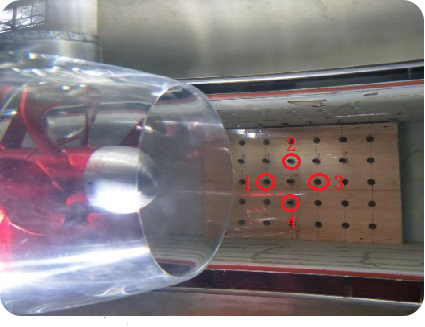
\includegraphics[scale=1.0]{3单级水听器布置.png}
    \caption{\label{fig:djstq}单级推进泵噪声试验中水听器布置}
\end{figure}
\subsection{推进泵噪声特性分析}
试验中通过固定叶轮转速、改变水洞流速的方法测量了进速系数0.3至1.2范围内,
对应固定转速为21rps,水速从1.26m/s增加至5.05m/s范围内10个工况点下的
水动力性能和噪声数据,本文选取进速系数分别为0.4,0.6,0.79,1.0和1.2,
对应水速分别为1.68m/s,2.52m/s,3.32m/s,4.2m/s和5.05m/s工况下的噪声数据进行分析。
基于噪声测试系统中的数据分析模块,获得了推进泵噪声的三分之一倍频程和频谱分析结果。

为了更好的表述推进泵噪声频谱的特性,本文对推进泵噪声频率的划分参考螺旋桨噪声的频率范围划分。
螺旋桨噪声频率范围的划分目前还没有统一的标准,其中
低频噪声通常在100Hz以下,也有一些研究将其
范围取为200-500Hz以下,高频噪声通常在1000Hz以上,而低频与高频之间过渡频
段的噪声也称为中频噪声。
本文将推进泵低频噪声的频率范围划分为100Hz以下,高频噪声在1000Hz以上,而低频与高频之间过渡频
段的噪声划分为中频噪声。

由于水听器所处的水舱为非消声环境,受壁面干涉等影响,所监测到的噪声信号干扰成分较多,对中低频噪声影响较大。
因此在对监测的推进泵噪声进行分析之前,本研究中测量了水洞空轴运转的背景噪声,将水速从1.02m/s增加至5.59m/s,
对该范围内的20个工况点进行了背景噪声的测量,分析了水速对背景噪声各频段的影响,进而评估水听器所处的非消声环境对
推进泵辐射噪声的干扰程度。
%因此在本文仅讨论水速对噪声各频段的影响,以及各频段噪声对噪声总声压级的贡献度。
\begin{figure}[htbp]
    \centering
    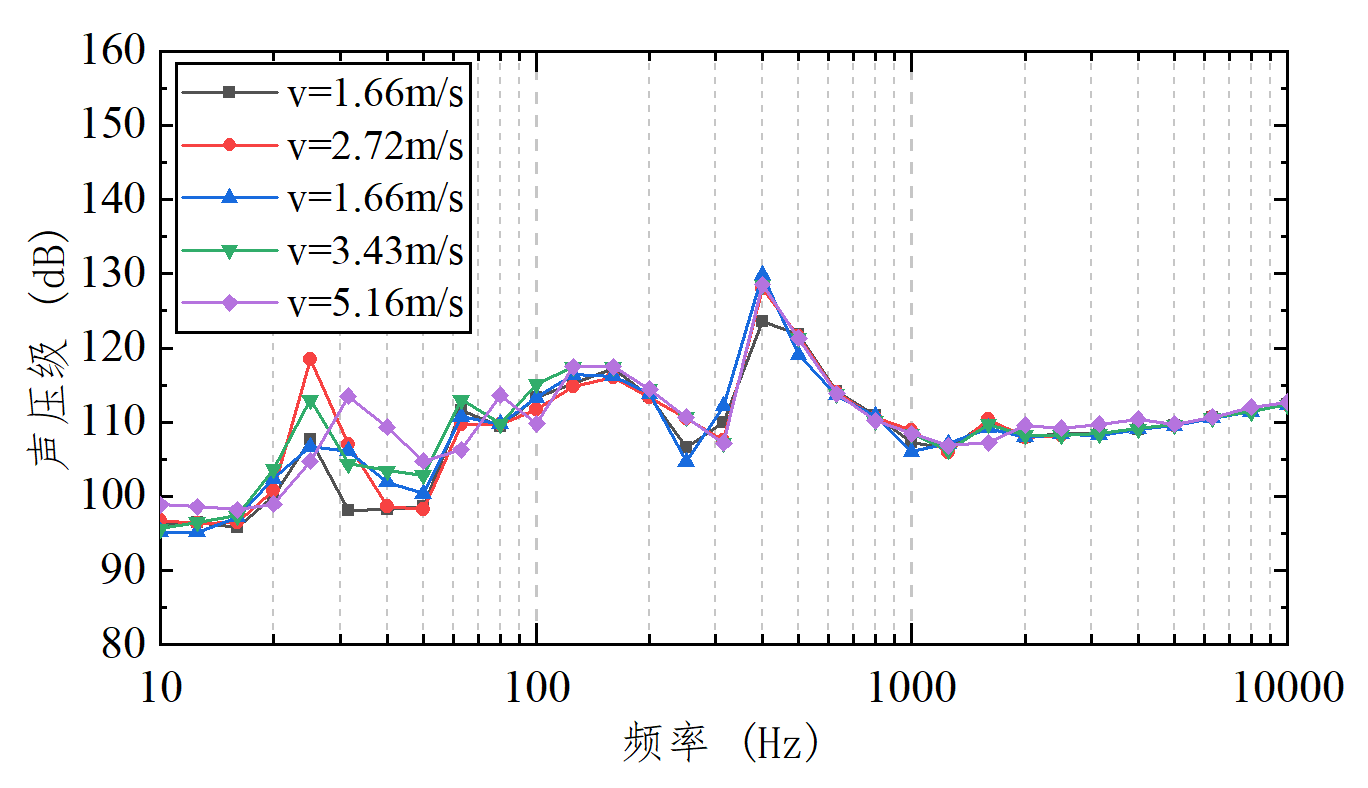
\includegraphics[scale=1]{3背景噪声的倍频程图.png}
    \caption{\label{fig:otcbeijing}水洞背景噪声1/3倍频程分析}
\end{figure}

如\autoref{fig:otcbeijing}所示为水洞背景噪声1/3倍频程图,可以看出水洞背景噪声能量在中低频段有明显波动,
高频段频谱平坦,单位频域下分布几近相同的能量密度,随着水速的增大,背景噪声各频段上的能量分布变化不大。
\begin{figure}[htbp]
    \centering
    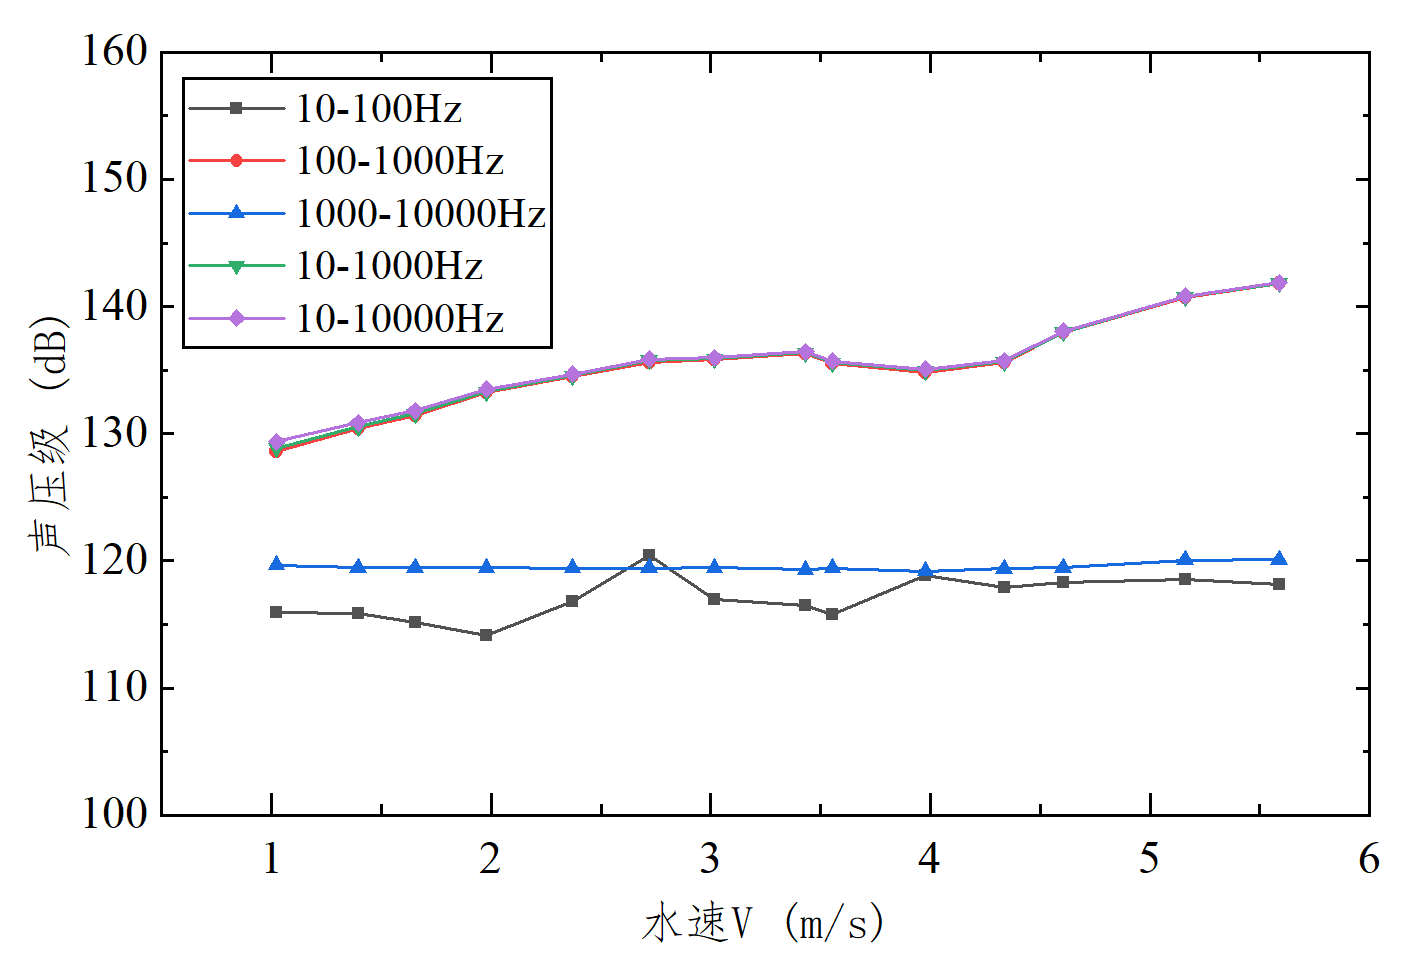
\includegraphics[scale=1]{3背景总声压级.png}
    \caption{\label{fig:beijingtotal}水洞背景噪声在不同水速下各个频段的噪声总声压级}
\end{figure}

如\autoref{fig:beijingfft}所示为水洞在水速为4.5m/s工况下的背景噪声频谱图,可以看出
频谱在低频段有丰富的线谱成分,从而影响该频段(10-100Hz)的能量密度分布。
频谱中300Hz线谱成分突出,为电磁干扰频率,显著影响了中频段(100-1000Hz)的能量。

\begin{figure}[htbp]
    \centering
    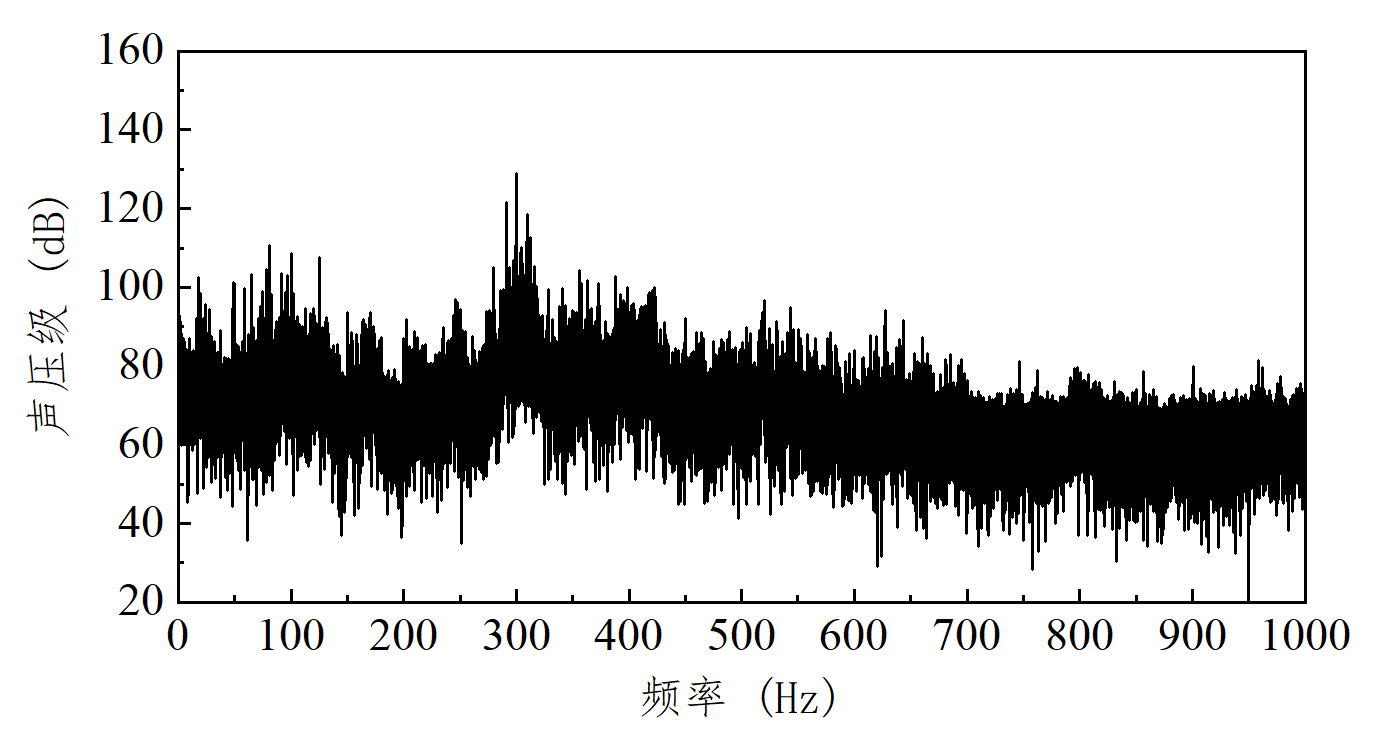
\includegraphics[scale=1]{3背景噪声频谱.png}
    \caption{\label{fig:beijingfft}v=4.5m/s工况下水洞背景噪声频谱}
\end{figure}

如\autoref{fig:beijingtotal}所示为水洞背景噪声在不同水速下各个频段,即在低频段(10-100Hz),
中频段(100-1000Hz),高频段(1000-10000Hz),中低频段(10-1000Hz)和全频段(10-10000Hz)的噪声总声压级,
从图中可以看出,随着水速的提升,低频段(10-100Hz)和高频段(1000-10000Hz)的声压级几乎没有发生变化。
中频段(100-1000Hz)、中低频段(10-1000Hz)和全频段(10-10000Hz)的变化曲线几乎重合,并且单调递增,
这说明中频段(100-1000Hz)噪声是背景噪声最主要的贡献量,水速的增大会提升中频段(100-1000Hz)的噪声能量,
进而增强背景噪声的总能量。
但是,水速的变化对中频段(100-1000Hz)和全频段(10-10000Hz)的总声压级影响较小,当水速从1.06m/s增大到
5.59m/s时,全频段(10-10000Hz)的总声压级的增幅仅为9.2dB。

以上分析表明,背景噪声的频谱呈现出中低频段宽带和线谱交叠的形貌,其300Hz线谱成分显著突出,
对推进泵噪声的影响体现在中低频段(10-1000Hz),因此在后文对推进泵噪声的分析中需要参考水洞背景噪声的频谱特性和
特征频段能量分布,剥离出背景噪声对推进泵噪声的干扰,探究水速对推进泵噪声各频段的影响,
以及各频段噪声对推进泵噪声总声压级的贡献度。

\begin{figure}[htbp]
    \centering
    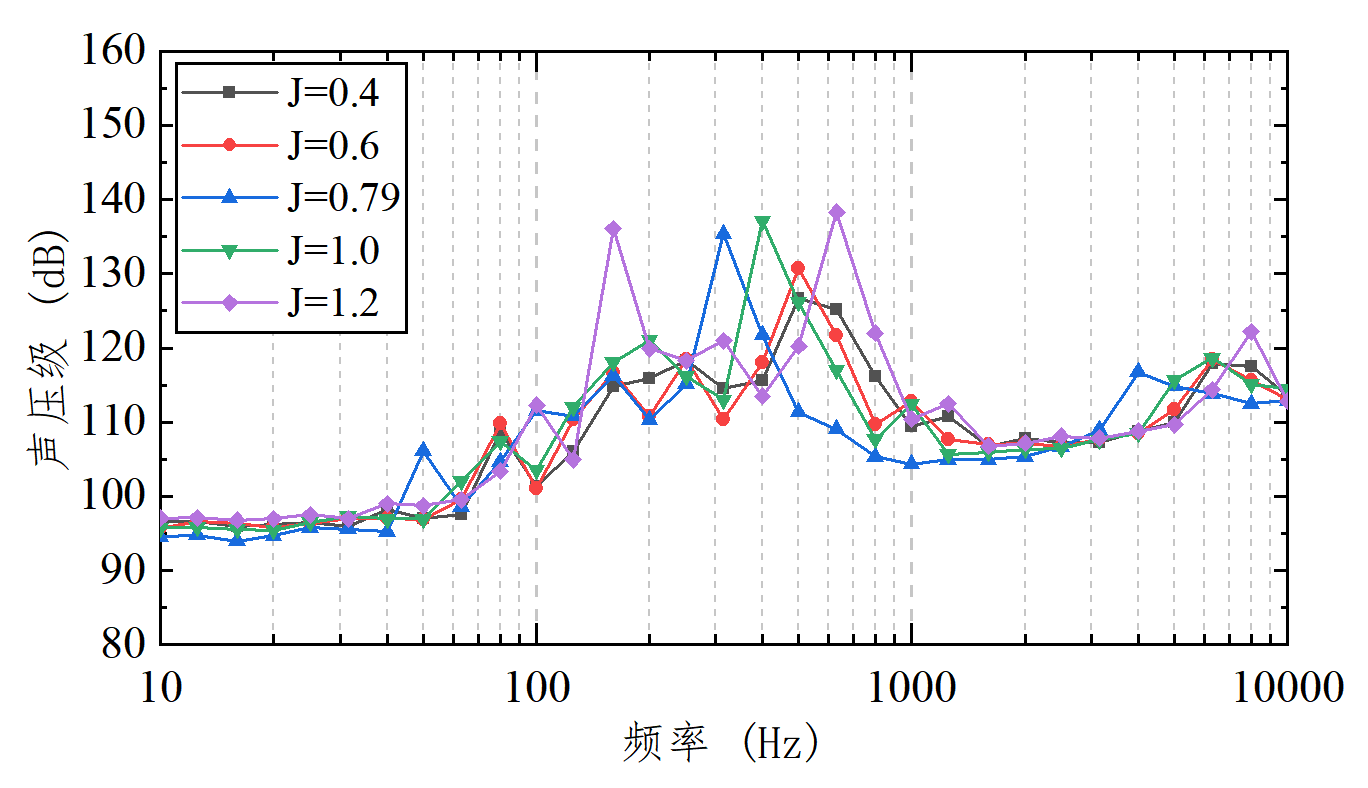
\includegraphics[scale=1]{3dj2_otc.png}
    \caption{\label{fig:djotc1}单级推进泵噪声1/3倍频程分析(1号传感器)}
\end{figure}
\begin{figure}[htbp]
    \centering
    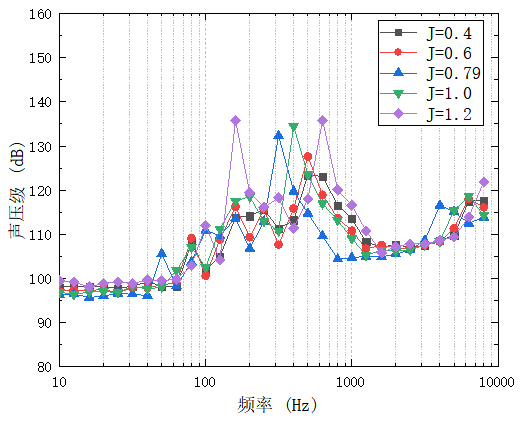
\includegraphics[scale=1]{3dj3_otc.png}
    \caption{\label{fig:djotc2}单级推进泵噪声1/3倍频程分析(2号传感器)}
\end{figure}
\begin{figure}[htbp]
    \centering
    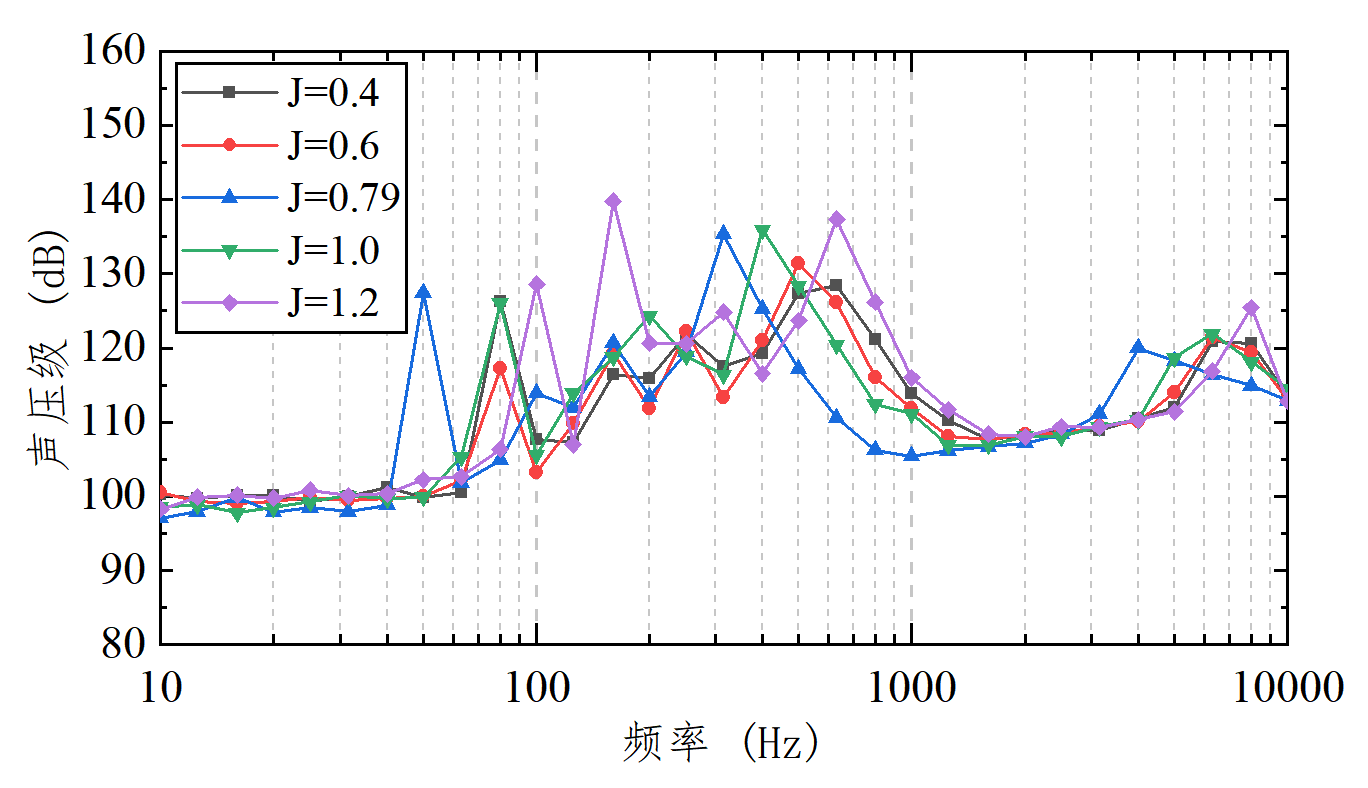
\includegraphics[scale=1]{3dj6_otc.png}
    \caption{\label{fig:djotc3}单级推进泵噪声1/3倍频程分析(3号传感器)}
\end{figure}
\begin{figure}[htbp]
    \centering
    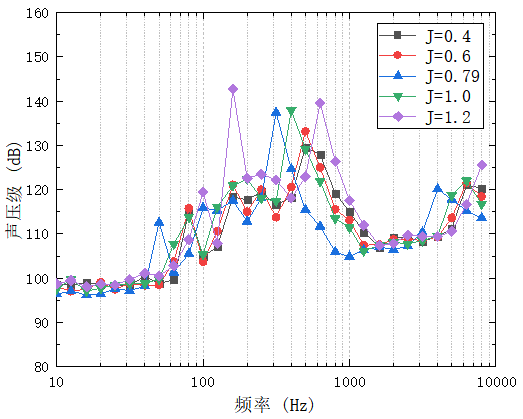
\includegraphics[scale=1]{3dj7_otc.png}
    \caption{\label{fig:djotc4}单级推进泵噪声1/3倍频程分析(4号传感器)}
\end{figure}

如\autoref{fig:djotc1},\autoref{fig:djotc2},\autoref{fig:djotc3},\autoref{fig:djotc4}所示,
分别为不同位置水听器在不同进速系数工况下的推进泵噪声的三分之一倍频程图。
从中可以发现,推进泵噪声能量主要集中在中低频段。
随着推进系数的增大,即水速的变大对中低频段有较大的影响,对高频频段的影响较小。
水速的变化对中低频段的影响体现在整个中低频宽带的频段上,而不是某个窄带特征频段。
水速的升高对中低频段的噪声影响较为复杂,没有明显的规律。
\begin{comment}
\begin{figure}[htbp]
        \centering
        \subfigure[pic1.]{
        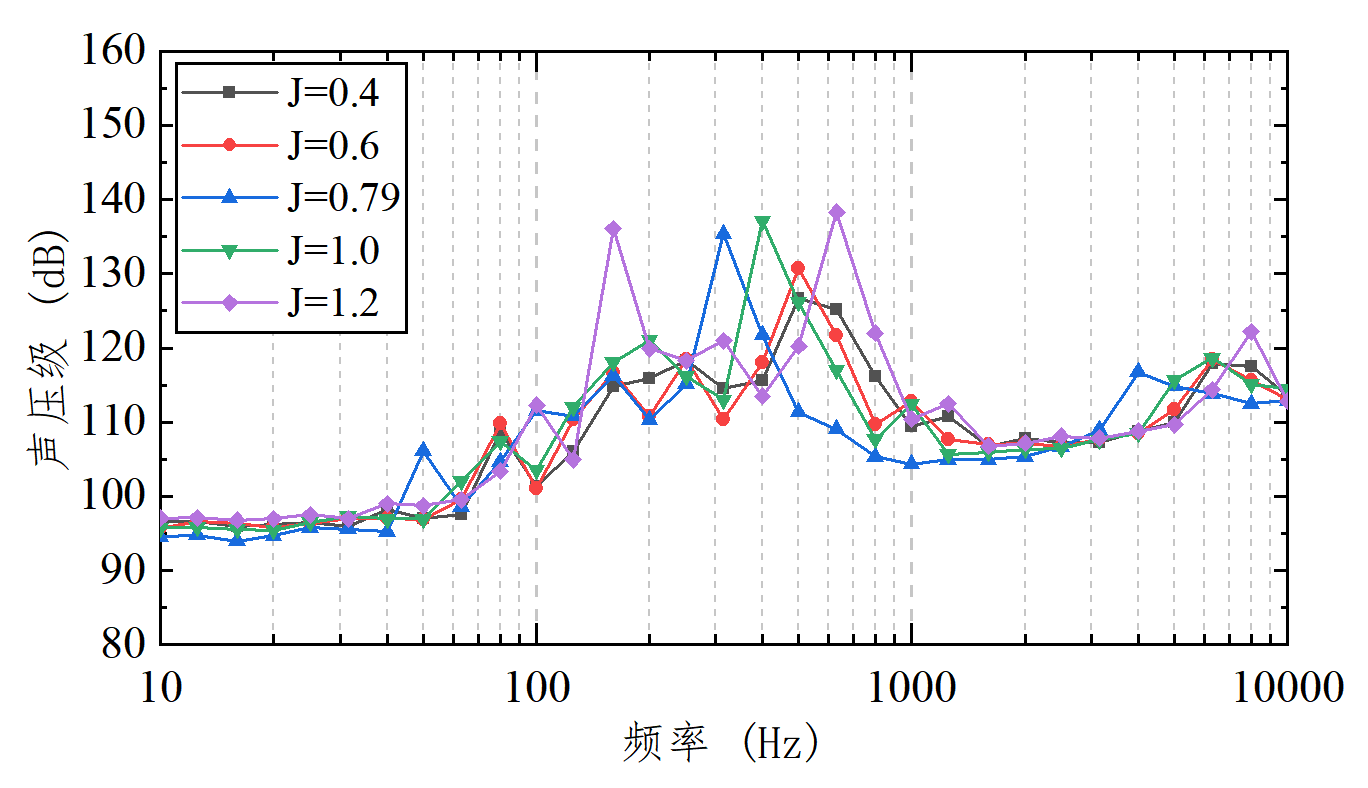
\includegraphics[scale=1.0]{3dj2_otc.png}
        }
\end{figure}
\addtocounter{figure}{-1}
\begin{figure}[htbp]
        \centering
        \addtocounter{figure}{1} 
        \subfigure[pic2.]{
        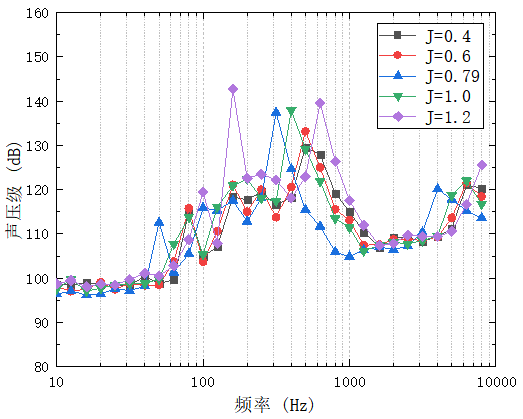
\includegraphics[scale=1.0]{3dj7_otc.png}
        }
        %\caption{\label{fig:dj_modle}不同进速系数下单级推进泵水下噪声三分之一倍频程图}
\end{figure}
\addtocounter{figure}{-1}
\begin{figure}[htbp]
        \centering
        \addtocounter{figure}{1} 
        \vspace{0.02cm}
        \subfigure[pic2.]{
        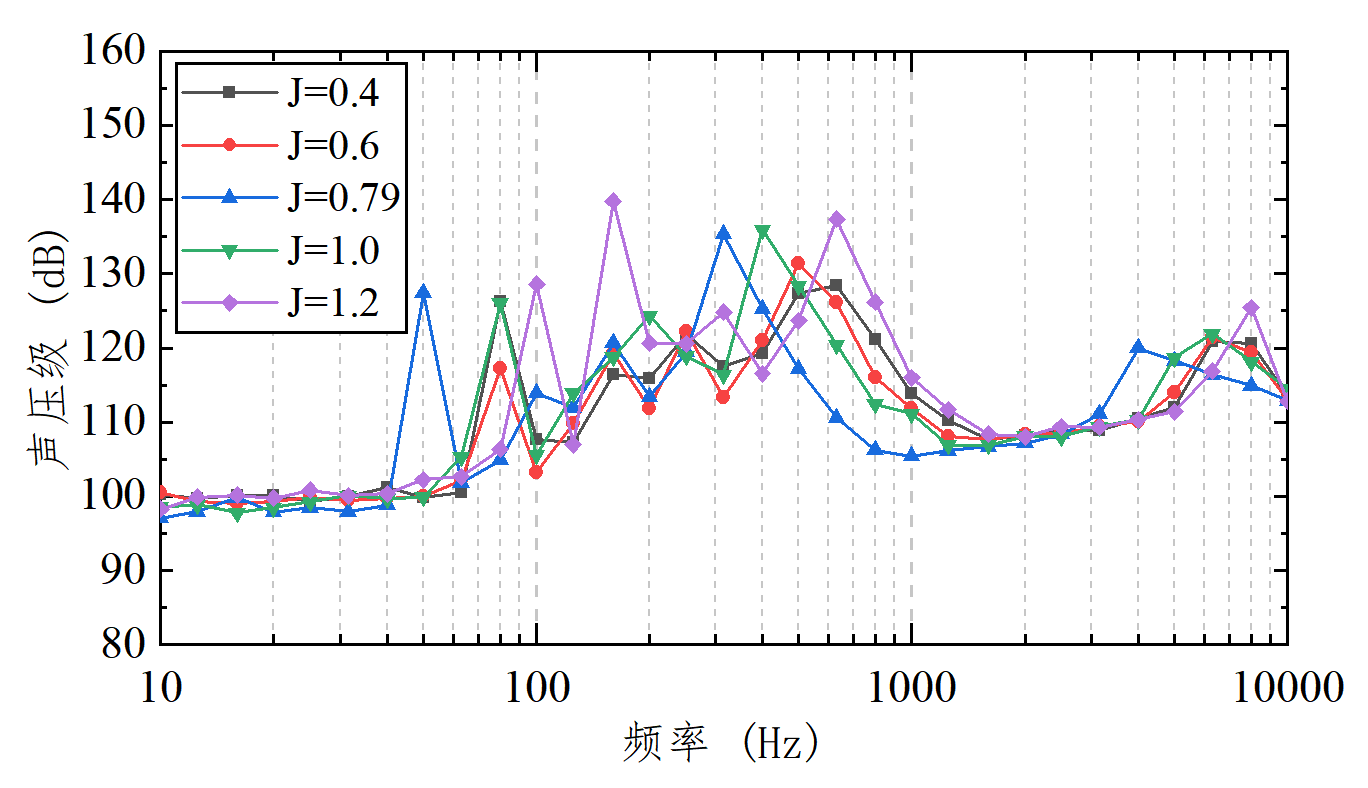
\includegraphics[scale=1.0]{3dj6_otc.png}
        }
        %\caption{\label{fig:dj_modle}不同进速系数下单级推进泵水下噪声三分之一倍频程图}
\end{figure}
\addtocounter{figure}{-1}
\begin{figure}[htbp]
        \centering
        \addtocounter{figure}{1} 
        \vspace{0.02cm}
        \subfigure[pic2.]{
        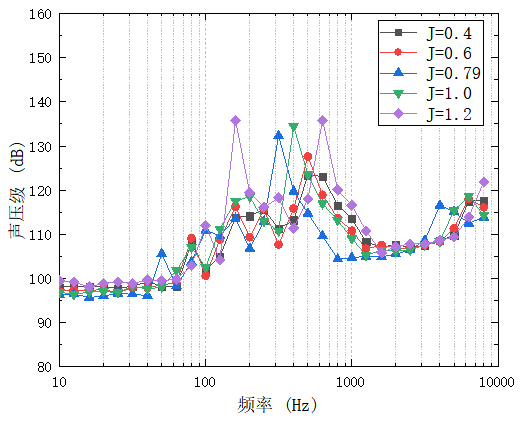
\includegraphics[scale=1.0]{3dj3_otc.png}
        }
        \caption{\label{fig:dj_modle}不同进速系数下单级推进泵水下噪声三分之一倍频程图}
\end{figure}
\end{comment}
\begin{figure}[htbp]
    \centering
    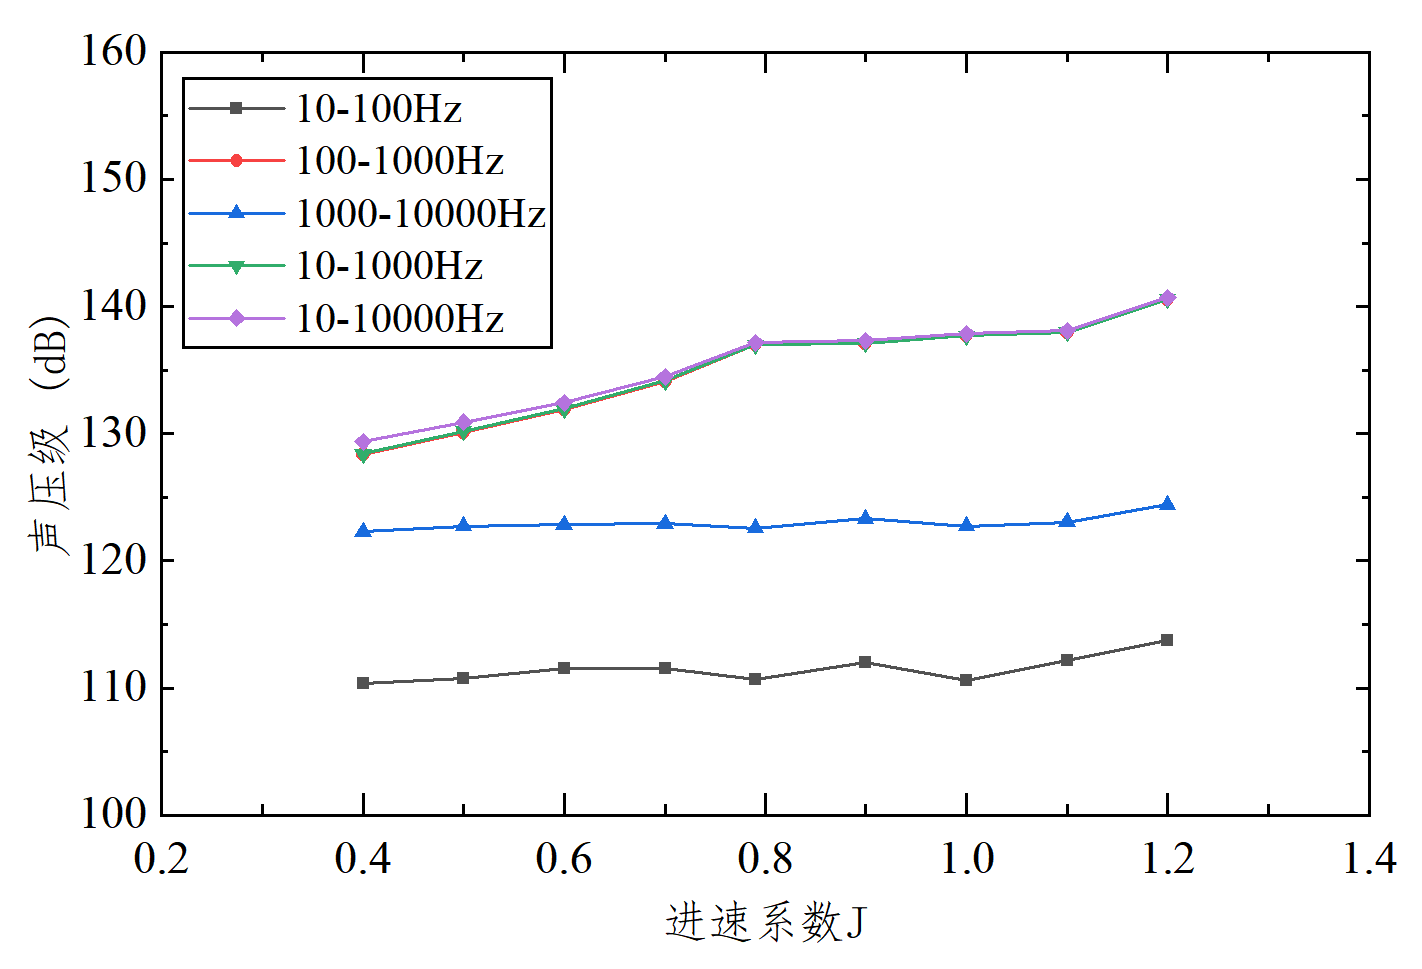
\includegraphics[scale=1]{3单级总声压.png}
    \caption{\label{fig:djtotal}单级推进泵噪声在不同进速系数下各个频段的噪声总声压级}
\end{figure}

为了进一步评估水速对推进泵特征频段的影响以及各个特征频段对噪声总级的贡献度,
基于噪声测试系统中的数据分析模块,可获得各测点平均以后,推进泵噪声在低频段(10-100Hz),
中频段(100-1000Hz),高频段(1000-10000Hz),中低频段(10-1000Hz)和全频段(10-10000Hz)的总声压级。
如\autoref{fig:djtotal}所示为推进泵噪声在不同进速系数下各个频段的噪声总声压级,
从图中可以看出,随着进速系数的变大,各个频段的声压级单调递增,
对比水洞背景噪声的特征频段分析,
说明水速的增大不仅会提升推进泵噪声低中高三个频段的能量,
还对全频段的声压级有增强作用。
其中,进速系数的变化对低频段(10-100Hz)和高频段(1000-10000Hz)的总声压级影响较小,当水速从1.26m/s增大到
5.05m/s时,低频段(10-100Hz)和高频段(1000-10000Hz)的总声压级的增幅分别为3.1dB和2.0dB。
水速对中频段(100-1000Hz)的总声压级影响更为显著,当水速从1.26m/s增大到5.05m/s时,
中频段(100-1000Hz)的总声压级增幅达到12.2dB。
不同进速系数下中频段(100-1000Hz)、中低频段(10-1000Hz)和全频段(10-10000Hz)的变化曲线几乎重合,
这说明中低频段噪声构成了推进泵噪声最主要的贡献量。

\begin{figure}[htbp]
    \centering
    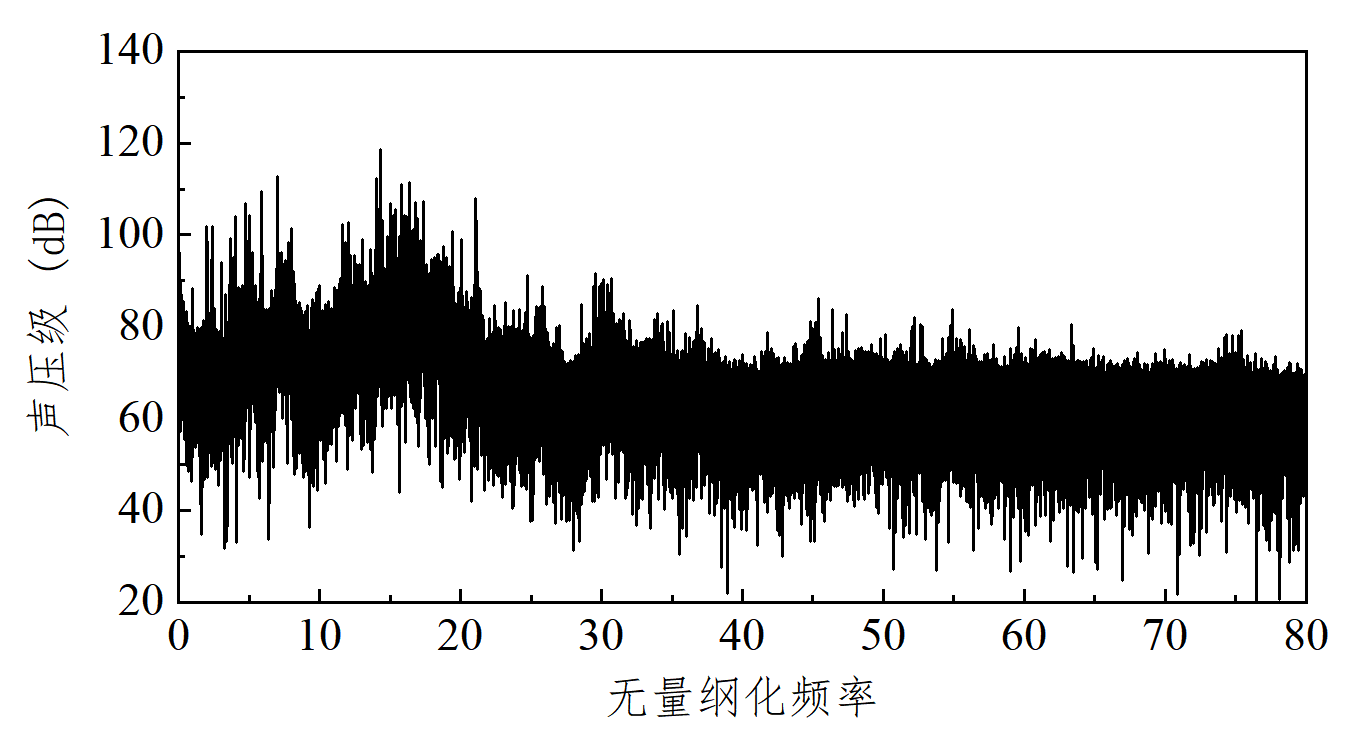
\includegraphics[scale=1]{3dj0.4频谱1.png}
    \caption{\label{fig:dj0.4}J=0.4进速系数下单级推进泵噪声频谱}
\end{figure}
\begin{figure}[htbp]
    \centering
    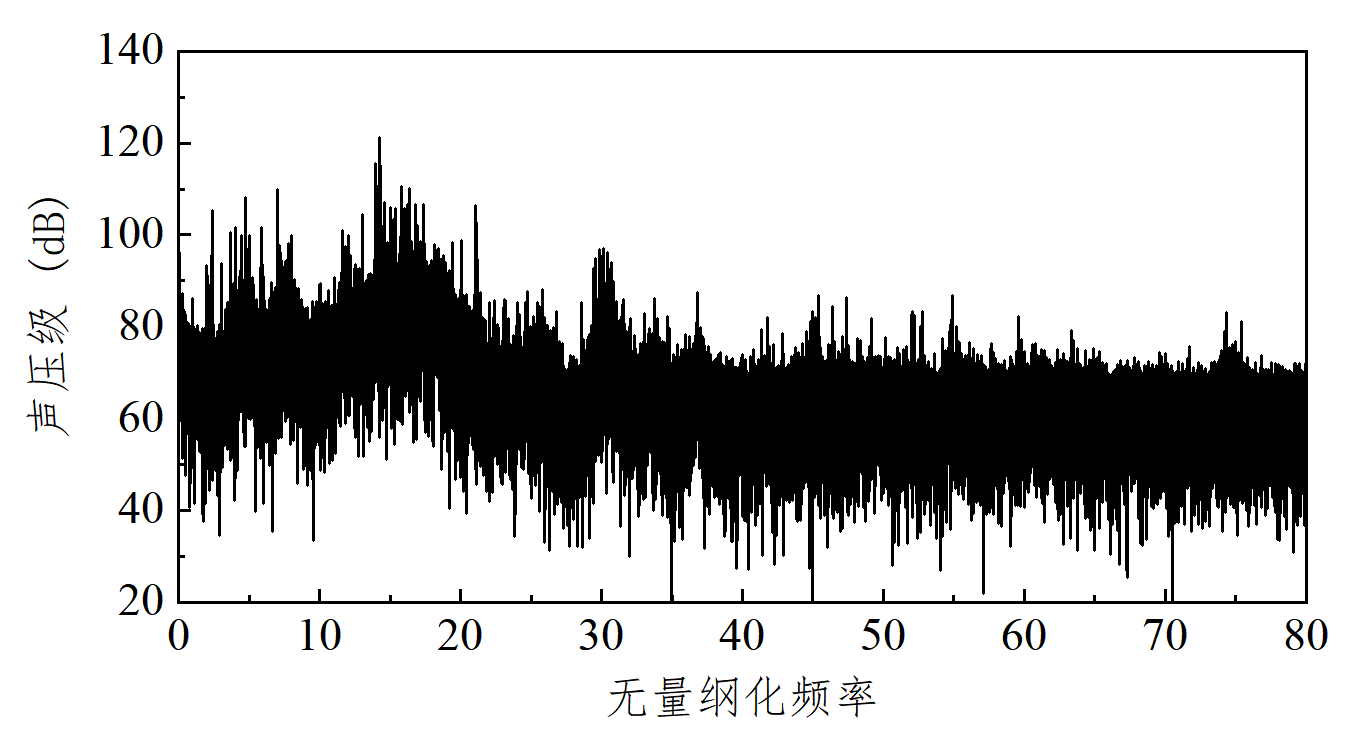
\includegraphics[scale=1]{3dj0.6频谱1.png}
    \caption{\label{fig:dj0.6}J=0.6进速系数下单级推进泵噪声频谱}
\end{figure}
\begin{figure}[htbp]
    \centering
    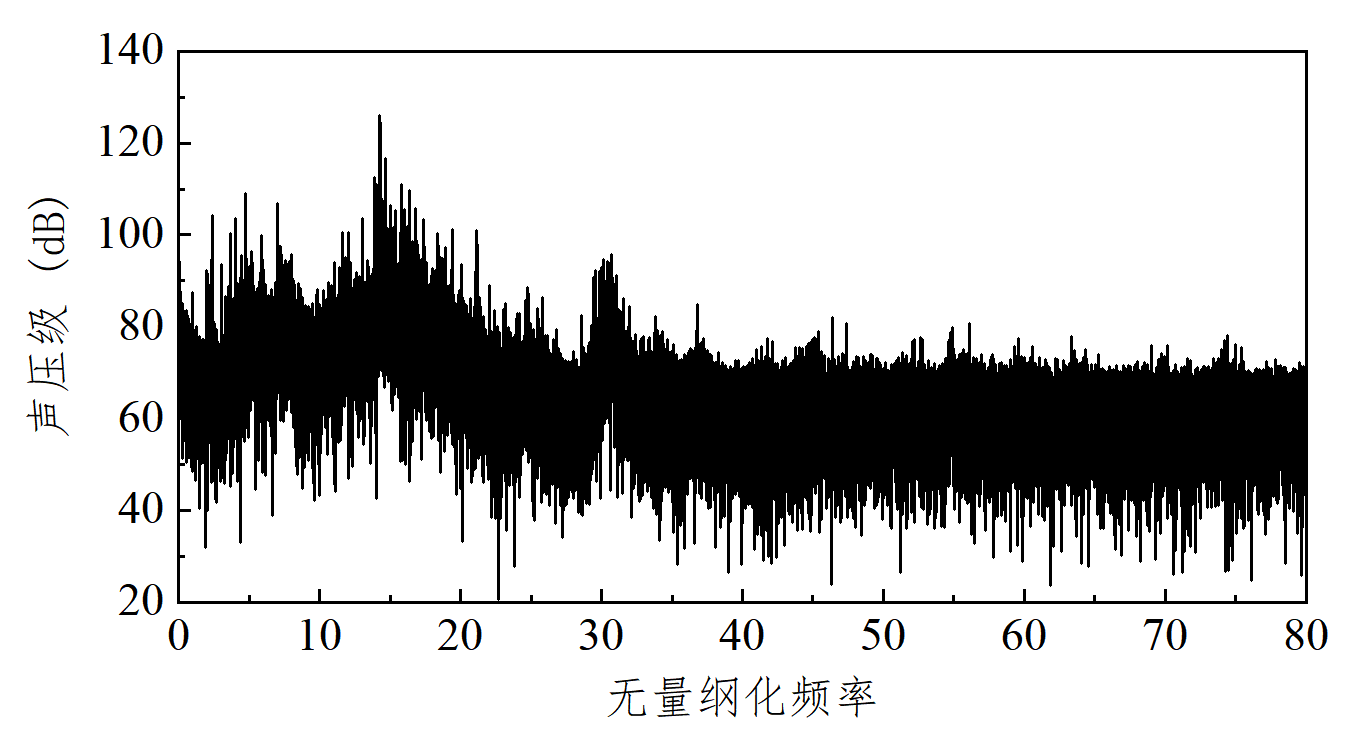
\includegraphics[scale=1]{3dj0.79频谱1.png}
    \caption{\label{fig:dj0.79}J=0.79进速系数下单级推进泵噪声频谱}
\end{figure}
\begin{figure}[htbp]
    \centering
    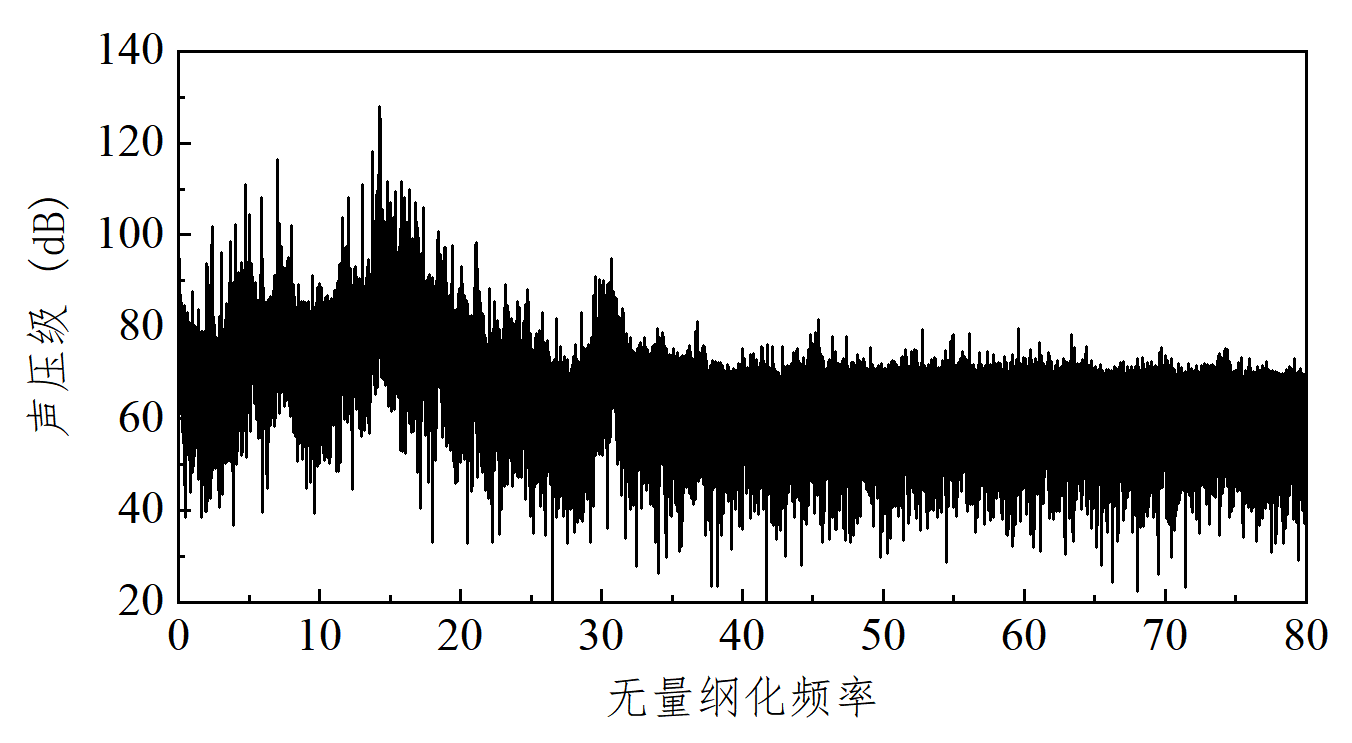
\includegraphics[scale=1]{3dj1.0频谱1.png}
    \caption{\label{fig:dj1}J=1.0进速系数下单级推进泵噪声频谱}
\end{figure}
\begin{figure}[htbp]
    \centering
    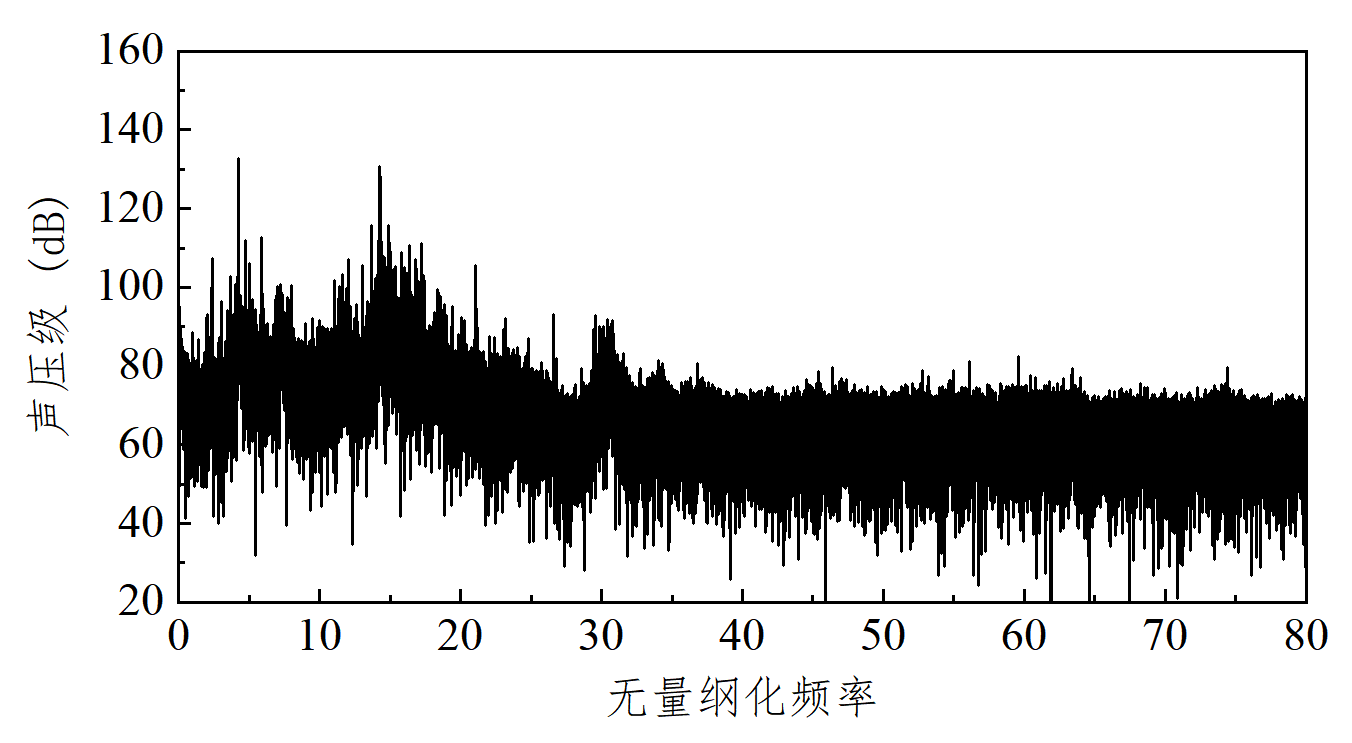
\includegraphics[scale=1]{3dj1.2频谱1.png}
    \caption{\label{fig:dj1.2}J=1.2进速系数下单级推进泵噪声频谱}
\end{figure}

试验结果中对频率作了无量纲化处理,即采用轴系转速进行无量纲化($f/f_n$),
随机选取了2号测点进行频谱特征分析。如\autoref{fig:dj0.4},\autoref{fig:dj0.6},
\autoref{fig:dj0.79},\autoref{fig:dj1},\autoref{fig:dj1.2}所示,
分别在不同进速系数工况下的单级推进泵噪声的频谱图。
可以看出监测到的推进泵噪声频谱特性表现为中低频宽带线
谱噪声和高频宽带谱噪声。
中低频段比较明显的线谱有7$f/f_n$(对应叶轮1阶叶频),14$f/f_n$(对应叶轮2阶叶频),21$f/f_n$(对应叶轮3阶叶频)。
在$f/f_n$-60$f/f_n$之间出现了连续的宽带线谱,包括以$f/f_n$为间隔的线谱成分,该频谱段表现出明显的调制特征。
除了这些特征线谱外,中低频段还有很多幅值不高的复杂线谱成分,
其中也包括水听器所处的非消声环境引起的干扰频率成分。
此外,轴频成分$f/f_n$几乎完全淹没在中低频段频谱中。

如\autoref{fig:dj0.4},\autoref{fig:dj0.6}所示,
在低水速工况下,频谱中的线谱频率成分复杂,特征频率如7$f/f_n$(对应叶轮1阶叶频)等成分淹没在宽带线谱中。
如\autoref{fig:dj1},\autoref{fig:dj1.2}所示,随着水速的增大,
14$f/f_n$(对应叶轮2阶叶频),21$f/f_n$(对应叶轮3阶叶频)等特征线谱成分显著突出。
\section{双级推进泵噪声特性的试验研究}
\subsection{推进泵试验模型}
本小节的研究对象是一种新型结构推进泵,该泵引入多级泵的设计思路,采用一根轴驱动两个叶轮,
再通过中间的导叶来回收环量。该双级推进泵通过采用特殊的两级叶轮形式降低推进器转速,提高能量密度。
其设计参数与上小节的单级推进泵都是根据某航行体的推进需求计算,并进行缩尺得到。
在单级推进泵的设计基础上,最终确定双级推进泵的轮缘直径为200mm,其直径空间与单级推进泵一致。
\begin{figure}[htbp]
    \centering
    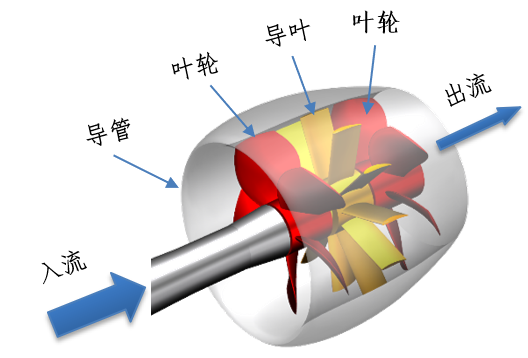
\includegraphics[scale=1.0]{5双级整体结构.png}
    \caption{\label{fig:sj_modle}双级推进泵设计模型}
\end{figure}

导管的设计选用 33 号减速喷管,可在一定程度上降低入流速度充分提升叶轮
的抗空化性能,并根据动量定理确定导管得出口直径,保证推进器能产生足够的推力。
叶轮的设计主要考虑了以下几个方面:
(1)在叶型剖面角度设计中,选用了较小的冲角,目的是在保证推进效率的前提下,更大程度地提高推进器的抗空化与声学性能;
(2)采用了较大的叶片落后角,可以使叶片在有限的轴向长度内具有更大的做功能力,以充分提升双级泵喷推进器的能量密度;
(3)中间导叶采用C型设计,可以有效地回收利用前叶轮出口的切向速度,并为后转子提供预旋,减小甚至消除推进系统出口的环量,以提高推进器的效率。
双级推进泵设计模型如\autoref{fig:sj_modle}所示。
\begin{table}[htbp]
    \centering
    \caption{\label{tab:sj}双级推进泵设计参数}
    \begin{tabular}{ccc}
     \toprule
     参数&值\\
     \midrule
     D(叶轮直径,mm)&200\\
     N(设计转速,rpm)&970\\
     L(导管长度,mm)&240\\
     $D_1$(入口直径,mm)&228\\
     $D_2$(出口直径,mm)&182\\
     $Z_1$(首级叶轮叶片数)&5\\
     $Z_2$(导叶叶片数)&11\\
     $Z_1$(首级叶轮叶片数)&6\\
     轮毂比&0.3\\
     旋向&右旋\\
     \bottomrule
    \end{tabular}
\end{table}

双级推进泵的设计参数如\autoref{tab:sj}所示。
\begin{figure}[htbp]
    \centering
    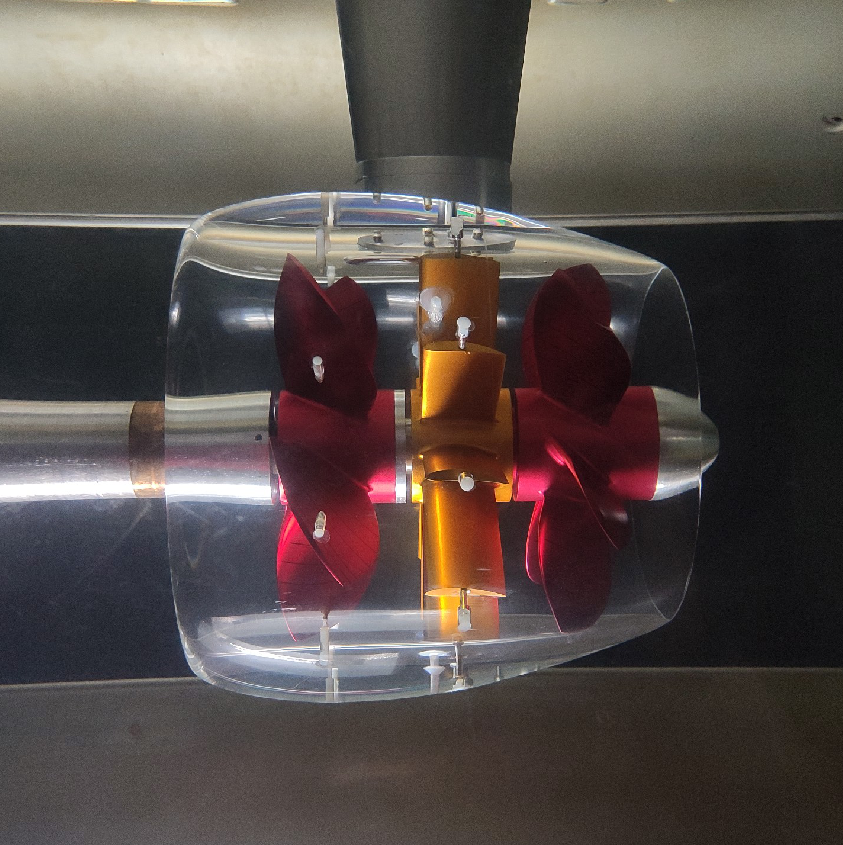
\includegraphics[scale=0.25]{3双级试验模型.png}
    \caption{\label{fig:sj_test}双级推进泵试验模型}
\end{figure}
推进器整体外形为流线型筒体,两级叶轮和导叶均装于筒体内。推进器前后两级叶轮位于导叶两侧,导叶体起到导流与支撑作用。
推进器叶轮采用铝合金加工制造,表面做阳极化处理。导管选用有机玻璃材质,表面做抛光处理,导管内壁与转叶叶梢间隙约1mm。
双级推进泵试验模型如\autoref{fig:sj_test}所示。
\begin{figure}[htbp]
    \centering
    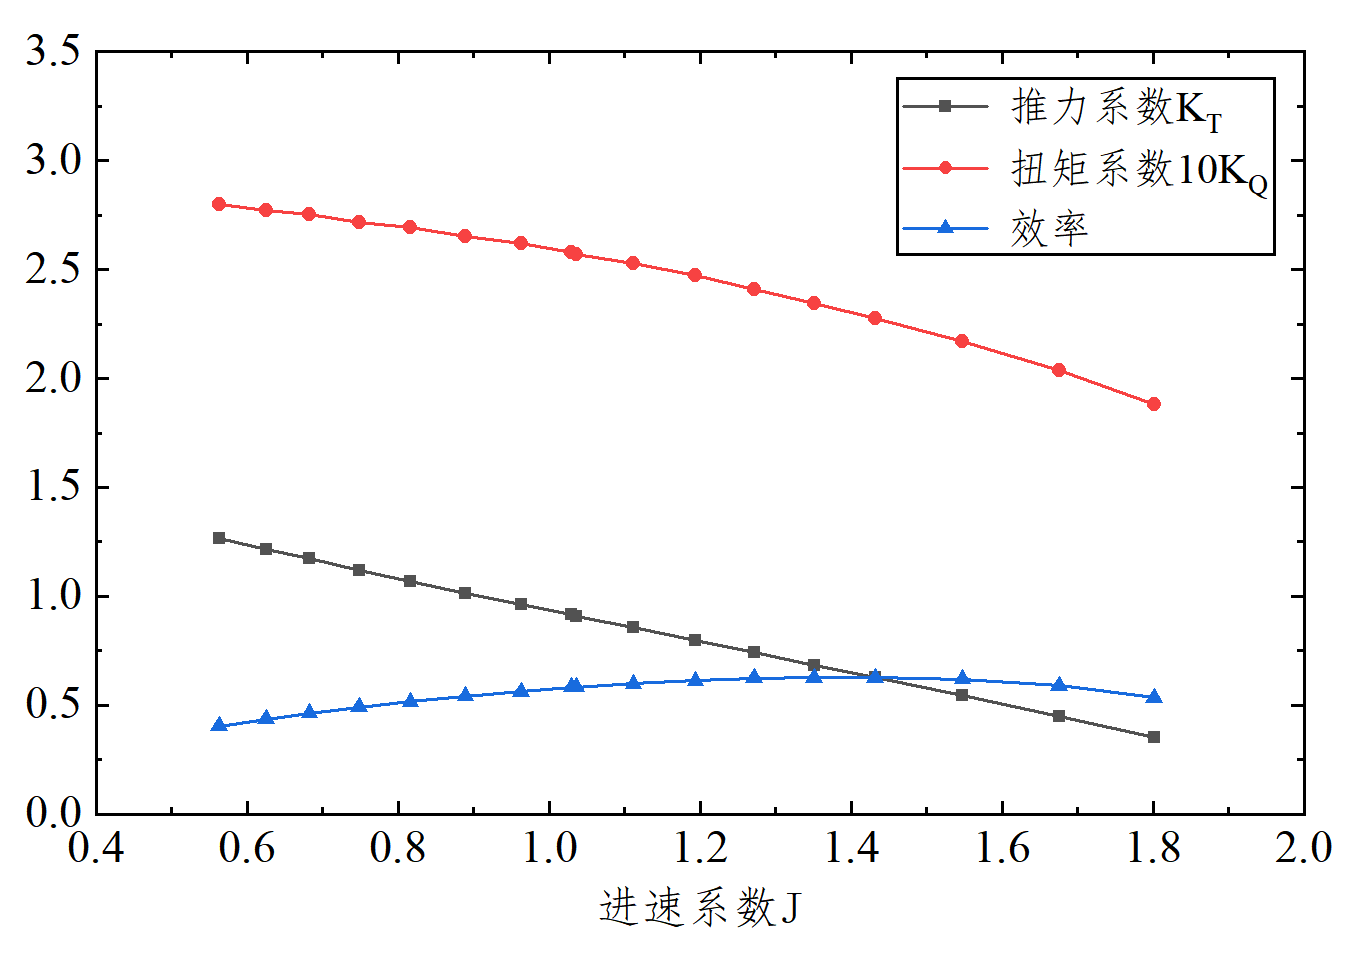
\includegraphics[scale=1]{3双级敞水性能.png}
    \caption{\label{fig:sj_changshui}双级推进泵敞水性能曲线}
\end{figure}

将水洞试验测得的双级推进泵推力、转矩和效率等数据无量纲化后,得到如\autoref{fig:sj_changshui}所
示的敞水性能曲线。从图中可以看出:随着进速系数J的增大,
推力系数$K_T$和转矩系数$K_Q$逐渐减小,而推进效率$\eta_0$先增大后减小,
并在 J=1.35 处有最大值 62.7\%。与常见的螺旋桨敞水性能
曲线相比,双级推进泵的敞水性能曲线随进速系数增加时变化趋势平缓,具有较高推进
效率的同时也有较宽的高效工作区。
推进器敞水性能曲线如\autoref{fig:sj_changshui}所示。
\begin{figure}[htbp]
    \centering
    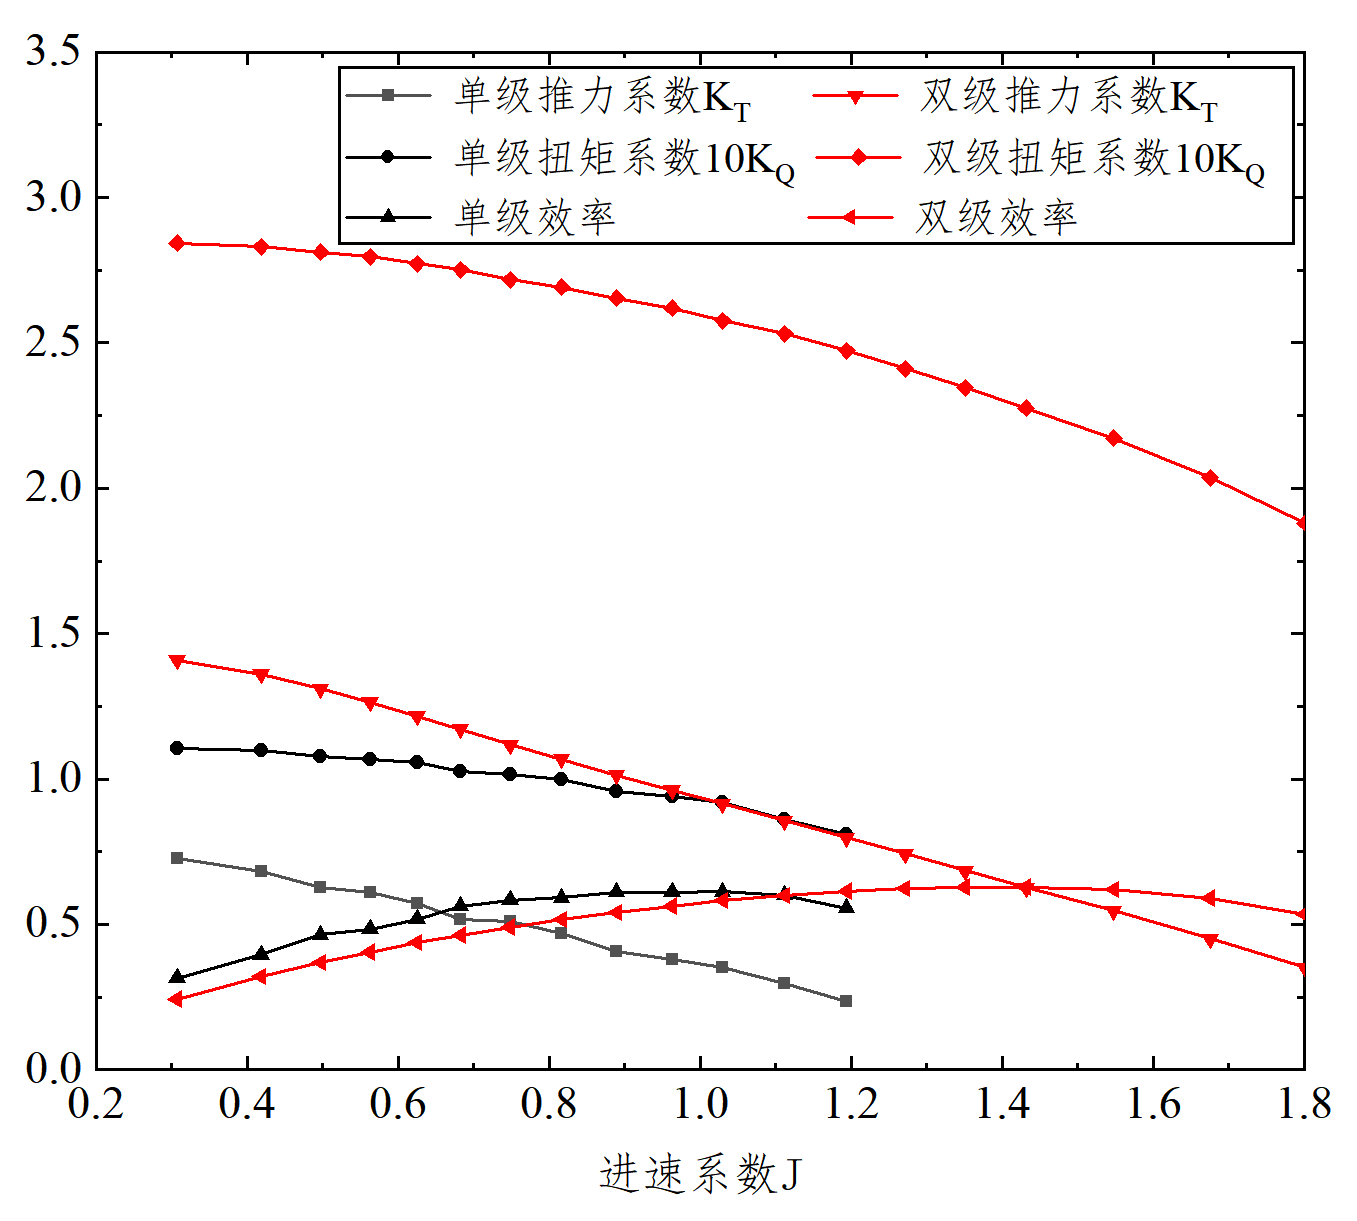
\includegraphics[scale=1]{3单双级敞水性能对比.png}
    \caption{\label{fig:sj_dj}双级推进泵与单级推进泵敞水性能曲线对比}
\end{figure}

与上小节研究的那台单级推进泵相比,两种推进泵的敞水性能曲线对比如\autoref{fig:sj_dj}所示。
在相同的直径空间下,双级推进泵的推力和转矩基本上相当于两台普通单级推进器。
此外,可以看到,单级推进泵的效率性能曲线在J=1.2的时候效率就开始下降了,而双级推进泵的效率性能曲线到1.8才开始下降,
双级推进泵的特性曲线变化更加平缓,这就使其高效区域更宽,
并且在高进速系数时仍可以保持较高效率,
说明双级推进器在高进速系数时仍可以保持较高效率,
有限的直径空间内,双级推进泵在降低转速的同时也有效提高了能量密度,适用于负荷较重的水面、水下航行器。


在噪声试验方面,采用水听器型号依旧为丹麦 Reson TC4013,采集装置也和单级推进泵一致,
利用水听器阵列进行推进泵辐射噪声的采集,其固定实验装置如\autoref{fig:sjstq}所示,
加工好的木板在水舱中与水洞侧壁面平行放置,水听器垂直置于木板孔中,
图上标号表示水听器的安放位置。基于噪声测试系统对上述位置的噪声信号进行同步采集,
采样频率为40960Hz,每次测试采样时间为10s。
\begin{figure}[htbp]
    \centering
    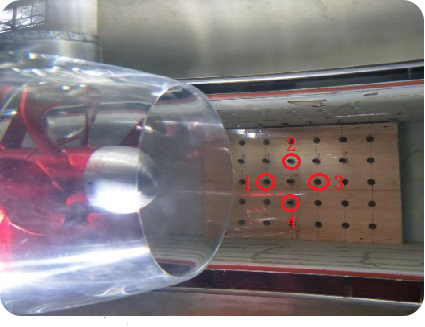
\includegraphics[scale=1.0]{3单级水听器布置.png}
    \caption{\label{fig:sjstq}双级推进泵噪声试验中水听器布置}
\end{figure}
\subsection{推进泵噪声特性分析}
试验中通过固定叶轮转速、改变水洞流速的方法测量了进速系数0.3至1.8范围内,
对应固定转速为16.66rps,水速从1.02m/s增加至6.01m/s范围内20个工况点下的
水动力性能和噪声数据,本文选取进速系数分别为0.5,0.8,1.0,1.3和1.5,
对应水速分别为1.68m/s,2.52m/s,3.32m/s,4.2m/s和5.05m/s工况下的噪声数据进行分析。
基于噪声测试系统中的数据分析模块,获得了推进泵噪声的三分之一倍频程和频谱分析结果。
本小节噪声范围的划分与单级推进泵保持一致,低频噪声的频率范围划分为100Hz以下,高频噪声在1000Hz以上,而低频与高频之间过渡频
段的噪声划分为中频噪声。

由于水听器所处的水舱为非消声环境,受壁面等影响,所监测到的噪声信号干扰成分较多,对中低频噪声影响较大。
因此在本文仅讨论水速对噪声各频段的影响,以及各频段噪声对噪声总声压级的贡献度。
\begin{figure}[htbp]
    \centering
    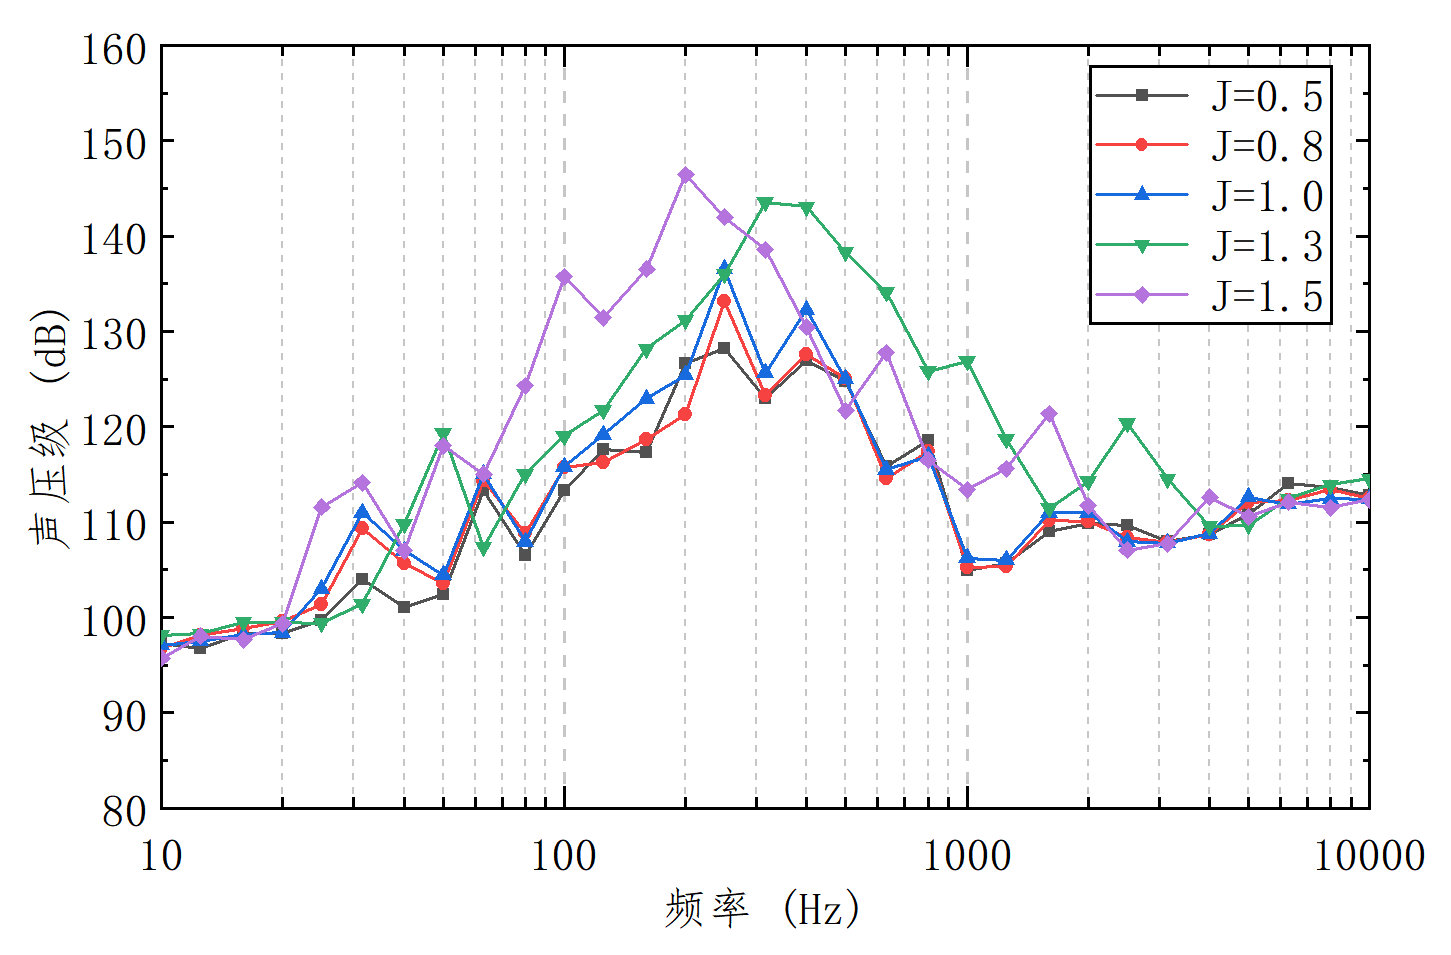
\includegraphics[scale=1]{3sj倍频程3.png}
    \caption{\label{fig:sjotc1}双级推进泵噪声1/3倍频程分析(1号传感器)}
\end{figure}
\begin{figure}[htbp]
    \centering
    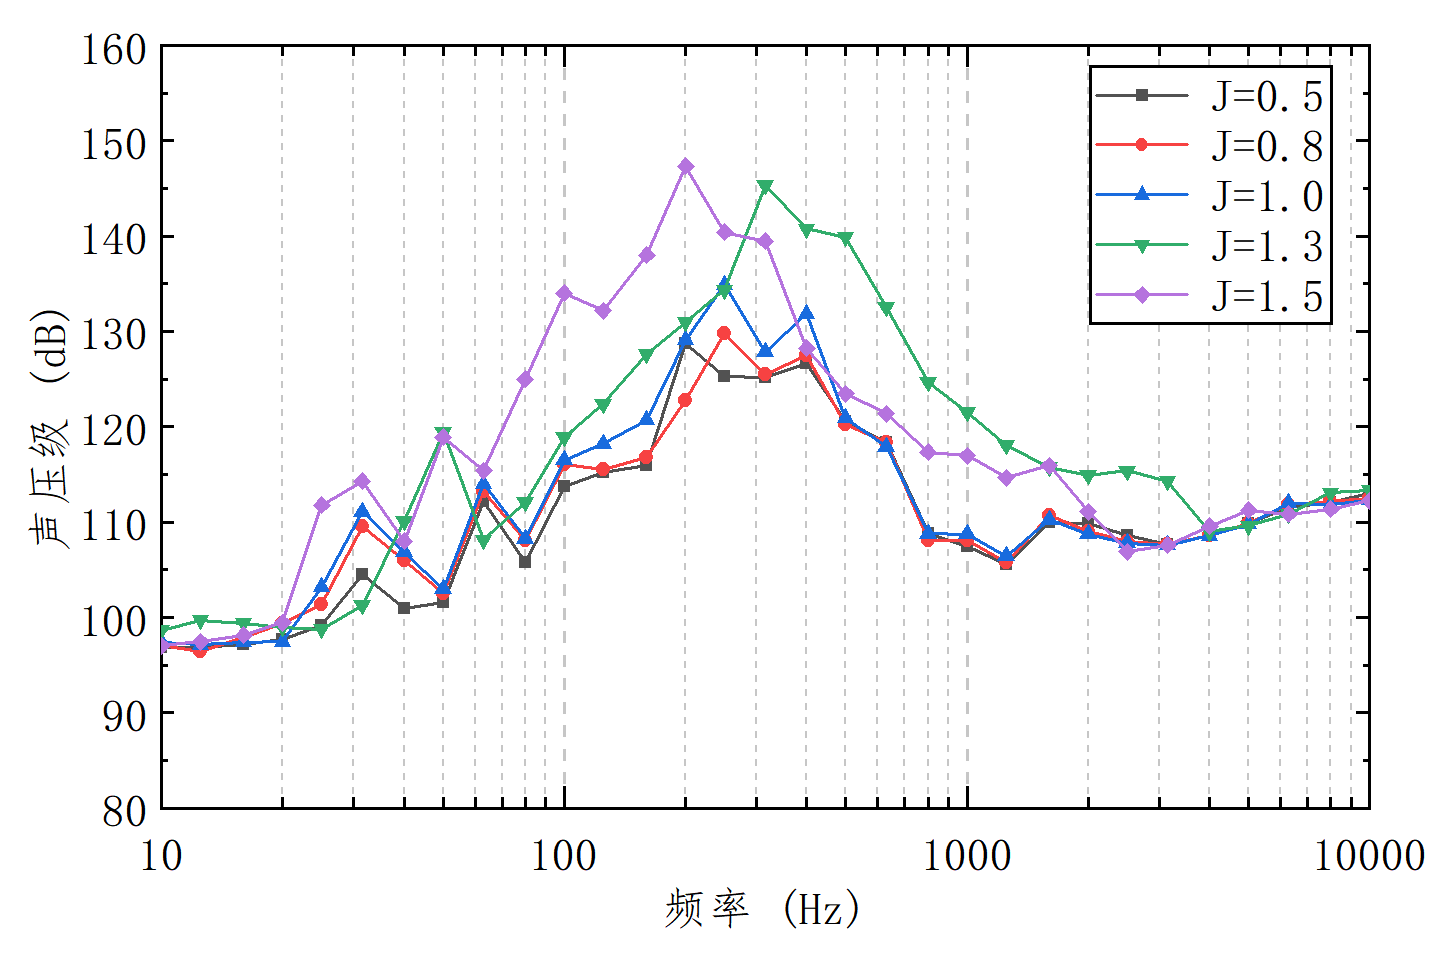
\includegraphics[scale=1]{3sj倍频程4.png}
    \caption{\label{fig:sjotc2}双级推进泵噪声1/3倍频程分析(2号传感器)}
\end{figure}
\begin{figure}[htbp]
    \centering
    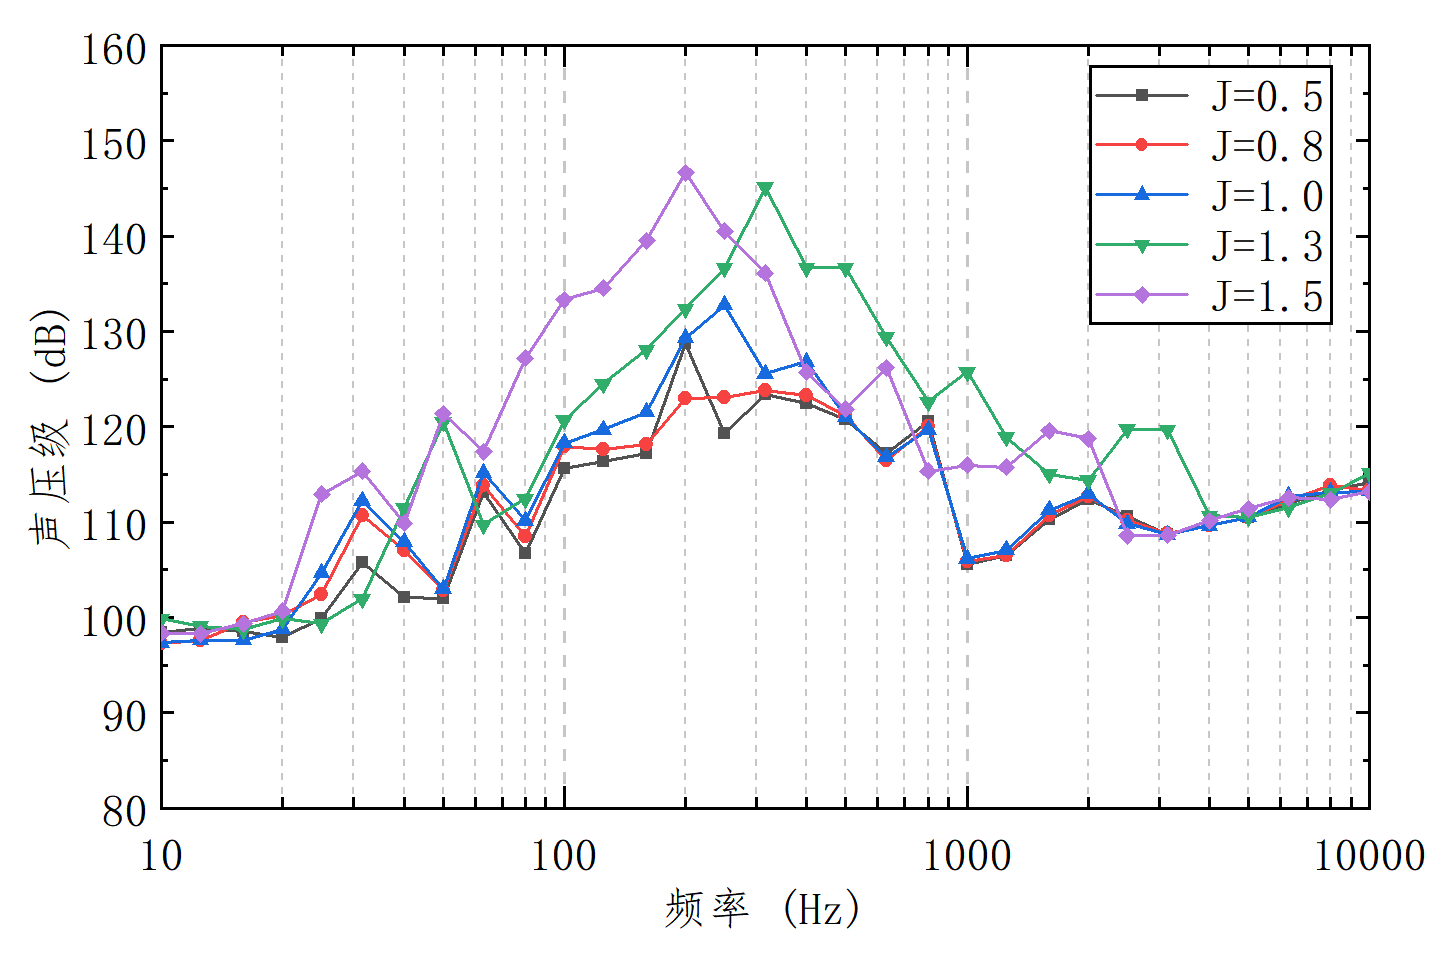
\includegraphics[scale=1]{3sj倍频程5.png}
    \caption{\label{fig:sjotc3}双级推进泵噪声1/3倍频程分析(3号传感器)}
\end{figure}
\begin{figure}[htbp]
    \centering
    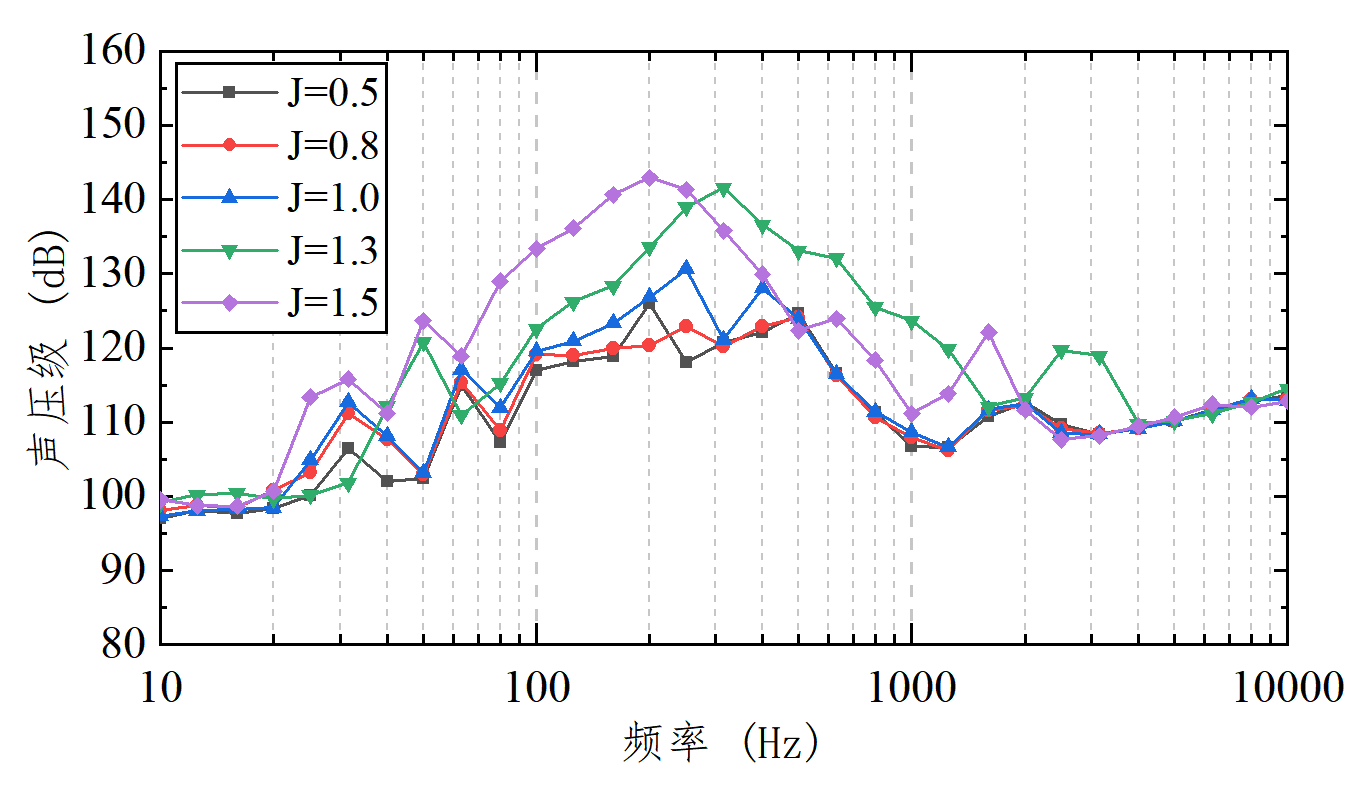
\includegraphics[scale=1]{3sj倍频程6.png}
    \caption{\label{fig:sjotc4}双级推进泵噪声1/3倍频程分析(4号传感器)}
\end{figure}

如\autoref{fig:sjotc1},\autoref{fig:sjotc2},\autoref{fig:sjotc3},\autoref{fig:sjotc4}所示,
分别为不同位置水听器在不同进速系数工况下的推进泵噪声的三分之一倍频程图。
随着推进系数的增大,即水速的变大对中低频段有较明显的影响,对高频频段的影响较小。
水速的变化对中低频段的影响体现在整个中低频宽带的频段上,同时,
水速的升高对中低频段的噪声有增强作用。
从中可以发现,所监测到的推进泵噪声能量主要集中在中低频段。
\begin{figure}[htbp]
    \centering
    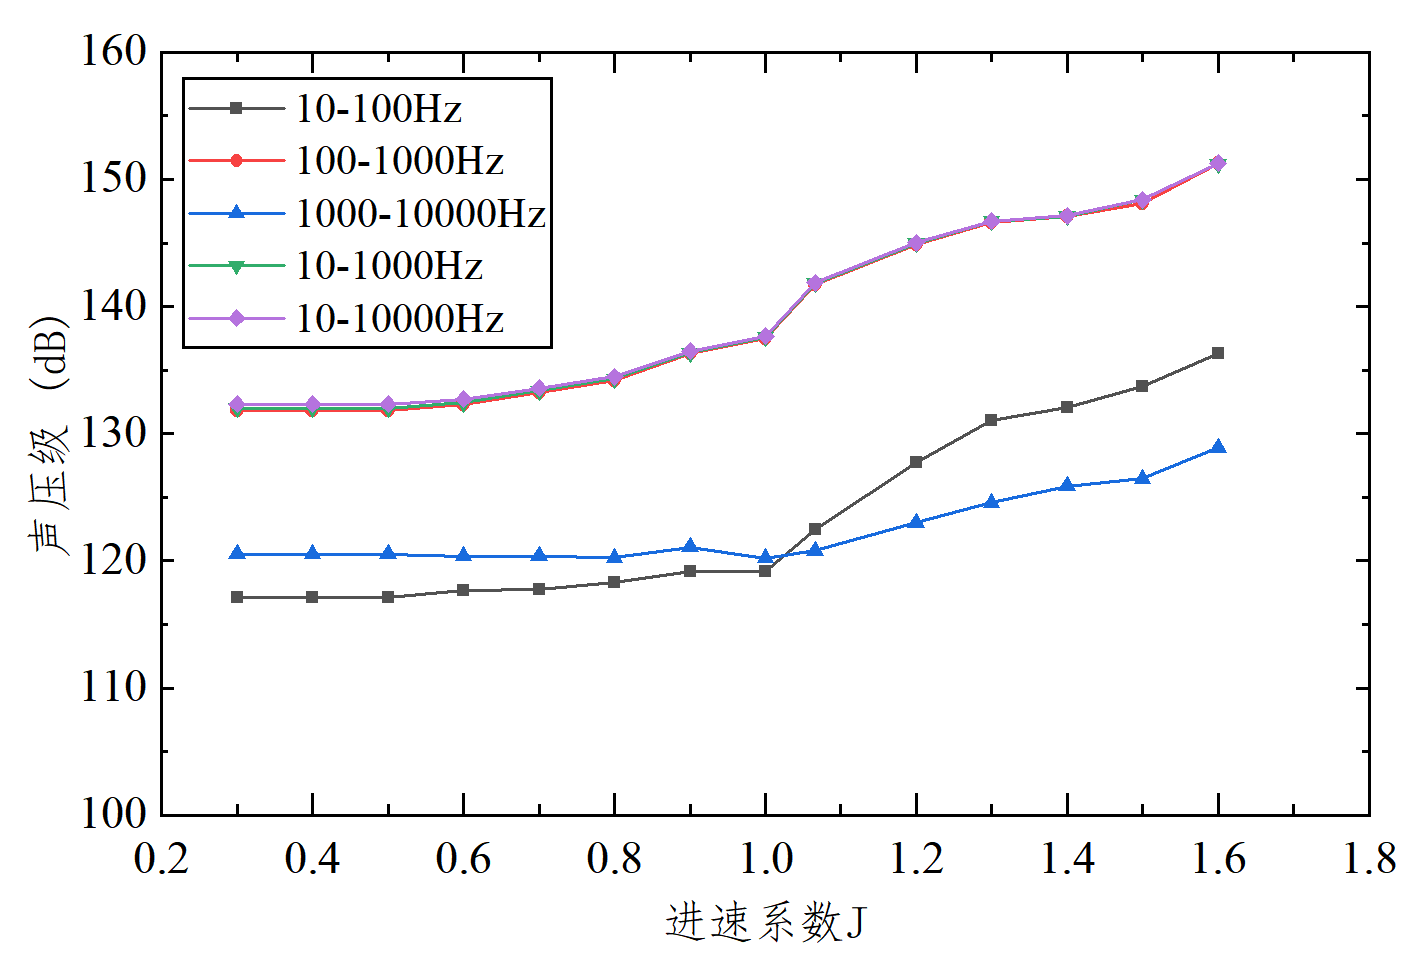
\includegraphics[scale=1]{3双级总声压级.png}
    \caption{\label{fig:djtotal}双级推进泵噪声在不同进速系数下各个频段的噪声总声压级}
\end{figure}

基于噪声测试系统中的数据分析模块,获得了各测点平均以后的推进泵噪声在低频段(10-100Hz),
中频段(100-1000Hz),高频段(1000-10000Hz),中低频段(10-1000Hz)和全频段(10-10000Hz)的总声压级。
如\autoref{fig:djtotal}所示为推进泵噪声在不同进速系数下各个频段的噪声总声压级,
可以看出,不同进速系数下中频段(100-1000Hz)、中低频段(10-1000Hz)和全频段(10-10000Hz)的变化曲线几乎重合,
这说明中低频段是推进泵噪声最主要的贡献量。
从图中可以看出,随着进速系数的变大,各个频段的声压级单调递增,
在水速变化的前半段,各频段的增长速率较为平缓,当水速达到3.4m/s以后,各频段的增长速率开始明显变大。
其中,进速系数的变化对低频段(10-100Hz)和高频段(1000-10000Hz)的总声压级影响较小,当水速从1.26m/s增大到
5.05m/s时,低频段(10-100Hz)和高频段(1000-10000Hz)的总声压级的增幅分别为8.4dB和9.1dB。
而进速系数对中频段(100-1000Hz)的总声压级影响更为显著,当水速从1.26m/s增大到5.05m/s时,
中频段(100-1000Hz)的总声压级增幅达到19.9dB。
说明水速的增大不仅会提升低中高三个频段的噪声能量,还对全频段的声压级有显著增强作用。

\begin{figure}[htbp]
    \centering
    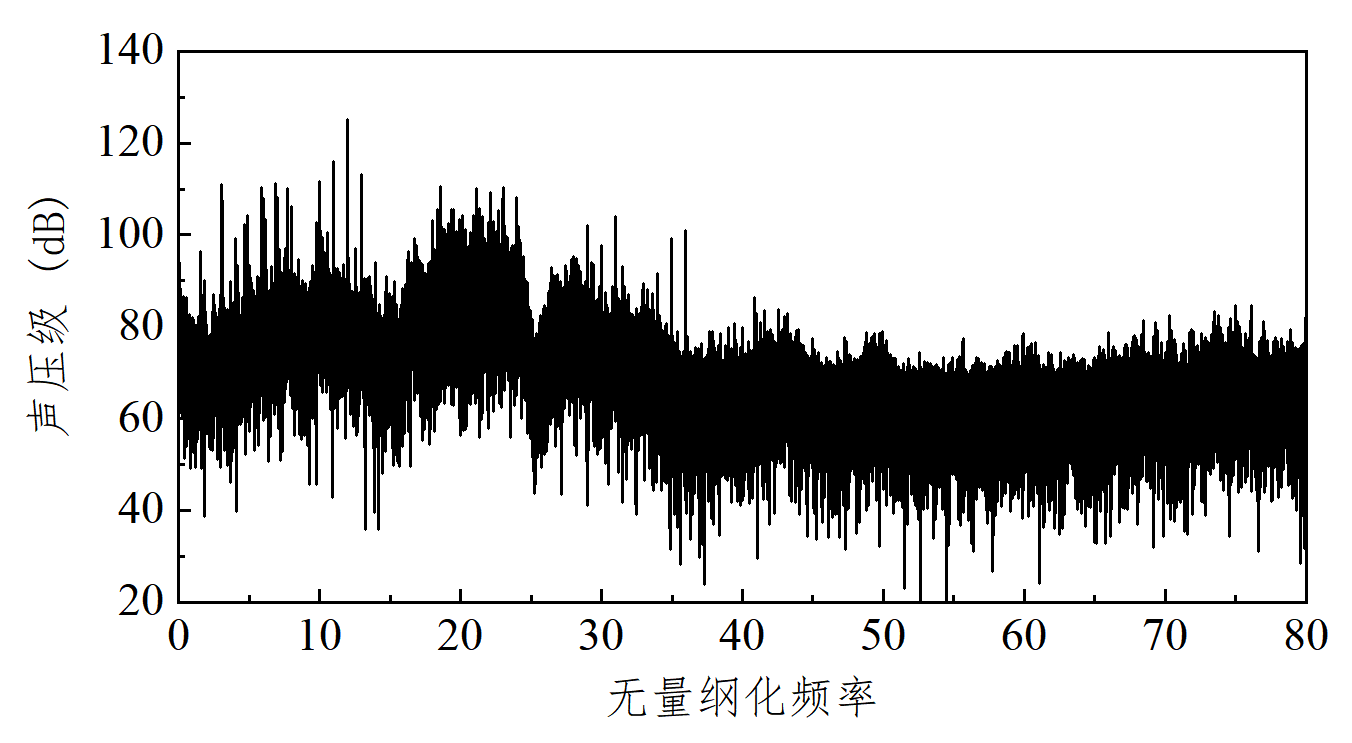
\includegraphics[scale=1]{3sj0.5频谱1.png}
    \caption{\label{fig:sj0.5}J=0.5进速系数下双级推进泵噪声频谱}
\end{figure}
\begin{figure}[htbp]
    \centering
    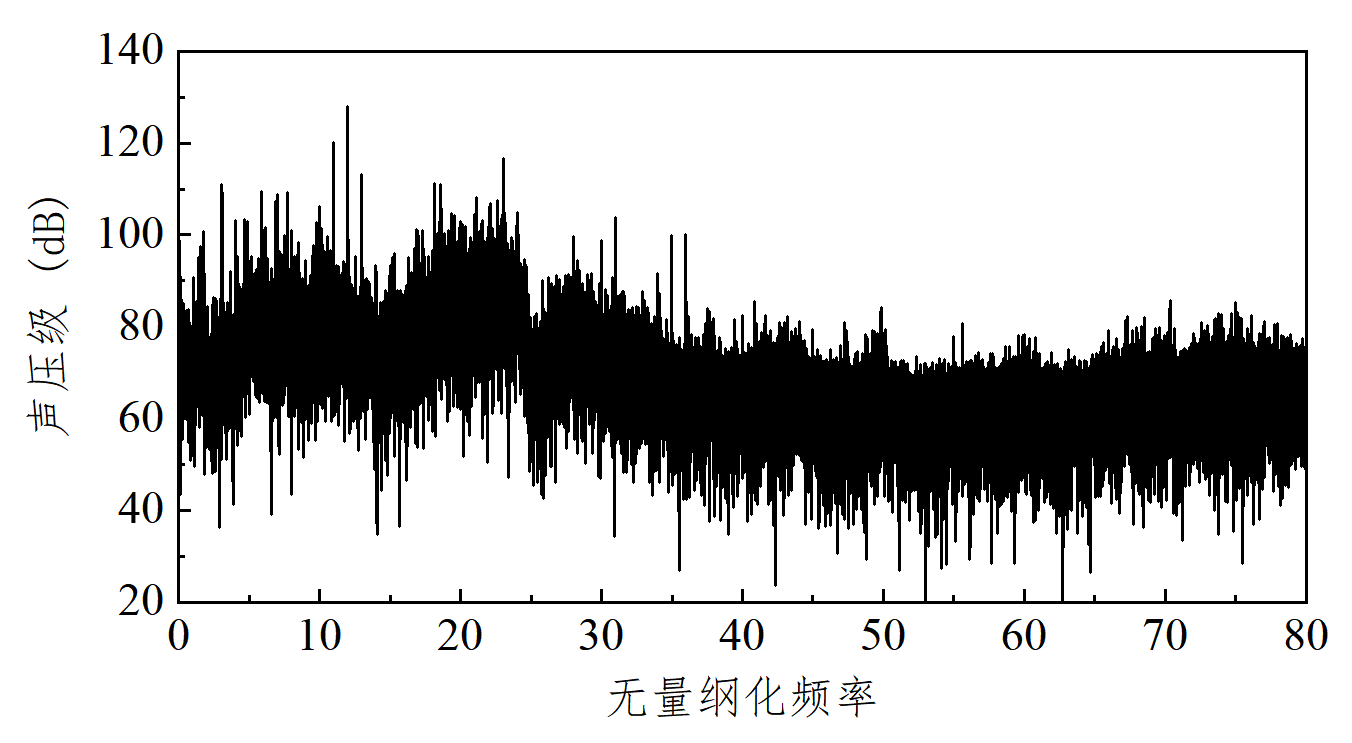
\includegraphics[scale=1]{3sj0.8频谱1.png}
    \caption{\label{fig:sj0.8}J=0.8进速系数下双级推进泵噪声频谱}
\end{figure}
\begin{figure}[htbp]
    \centering
    \includegraphics[scale=1]{3sj1.0频谱1.png}
    \caption{\label{fig:sj1.0}J=1.0进速系数下双级推进泵噪声频谱}
\end{figure}
\begin{figure}[htbp]
    \centering
    \includegraphics[scale=1]{3sj1.3频谱1.png}
    \caption{\label{fig:sj1.3}J=1.3进速系数下双级推进泵噪声频谱}
\end{figure}
\begin{figure}[htbp]
    \centering
    \includegraphics[scale=1]{3sj1.5频谱1.png}
    \caption{\label{fig:sj1.5}J=1.5进速系数下双级推进泵噪声频谱}
\end{figure}

试验结果中对频率作了无量纲化处理,即采用轴系转速进行无量纲化($f/f_n$),
随机选取了2号测点进行频谱特征分析。如\autoref{fig:dj0.4},\autoref{fig:dj0.6},
\autoref{fig:dj0.79},\autoref{fig:dj1},\autoref{fig:dj1.2}所示,
分别在不同进速系数工况下的双级推进泵噪声的频谱图。
监测到的推进泵噪声频谱特性表现为中低频宽带与线
谱噪声交叠和高频宽带的形貌。
可以看出,中低频段中比较明显的线谱有5$f/f_n$(对应首级叶轮1阶叶频),6$f/f_n$(对应次级叶轮1阶叶频),
9$f/f_n$,10$f/f_n$(对应首级叶轮2阶叶频),11$f/f_n$(对应导叶1阶叶频),12$f/f_n$(对应次级叶轮2阶叶频),23$f/f_n$。
在$f/f_n$-60$f/f_n$之间出现了连续的宽带线谱,包括以$f/f_n$为间隔的线谱成分,该频谱段表现出明显的调制特征。
除了这些特征线谱外,中低频段还存在丰富的复杂线谱成分,
其中也包括水听器所处的非消声环境引起的干扰频率成分。
此外,轴频成分$f/f_n$完全淹没在中低频段频谱中。

随着水速的增大,宽带线谱特征更加显著,频谱能量愈发集中在10$f/f_n$-15$f/f_n$之间的宽带频段,
尤其是10$f/f_n$(对应首级叶轮2阶叶频),11$f/f_n$(对应导叶1阶叶频),12$f/f_n$(对应次级叶轮2阶叶频)
等特征线谱成分显著突出。
\section{本章小结}
\chapter{基于循环平稳分析方法的推进泵噪声信号模型研究}
\section{引言}
推进泵噪声按声源类型的不同,可以将推进泵噪声分为流致噪声和振动噪声,其中流致噪声是推进泵噪声的主要贡献者。
流致噪声是由泵内非定常流动与泵相互作用产生的非定常流致激励所引起的,
前期研究发现,推进泵叶轮与其他部件之间的动静干涉是重要的流致噪声激励源。
动静干涉是指由于推进泵转子(如叶轮)和静止部件(如导叶和导管)之间的周
向不均匀流动在旋转过程中相互作用,从而导致了泵内部流道中复杂的非定常流动现象。
因此,推进泵噪声是推进泵流致激励特性的最直接的外在表现,
构建推进泵流致激励源特征提取的有效方法和途径,从噪声信号中分析出流致激励源
的影响程度以及两者的作用机理,对于推进泵低噪声设计及发展噪声能量主动控制技术至关重要。

第三章推进泵噪声试验结果显示,监测到的推进泵噪声频谱特性表现为中低频线谱噪声,中低频宽带谱噪声和
高频宽带谱噪声。
噪声信号中蕴含着丰富的流致激励源信息,但是难以从噪声信号频谱中提取出流致激励源特征信号,信号中存在复杂的干扰因素:
其一,推进泵处在复杂的背景环境声场中,背景声场中存在复杂的干扰
成分,影响测试系统对推进泵目标真实辐射噪声信号的监测;其二,推进泵结构复杂,
由于具有周期性分布的旋转、静止构件和导管,
辐射噪声的声源构件并不单一,其辐射噪声具有分量复杂性。
基于上述干扰因素,监测系统接收到的目标声场信号的
信噪比较低,特征信号如动静干涉频率、轴频等与其他背景噪声相比均较为微弱,给基于传统噪声特征提取方法带来了困难,
难以准确的获得推进泵的工作状态和结构信息,也给流致激励源特征的提取带来很大的难度。

其次,推进泵流致噪声存在显著的调制现象,上章节的推进泵噪声频谱已呈现出较强的调制特性,
调制现象也是流致激励作用的结果,其中蕴含着丰富的流致激励源信息,
但是传统的频谱分析及解调方法无法实现高精度低频调制特征的提取。
因此,针对推进泵噪声信号的特点,开展对其噪声信号的分量分析研究,
基于其信号的循环平稳特性,
建立流致激励源-噪声信号模型,
探索合适的流致激励源特征提取方法,对噪声的机理分析和流致激励源特征提取有重要意义。
\section{推进泵噪声信号分量分析}
推进泵由于其具有运转模式的周期性,具有明显的调制特性。从信号组成成分来看,推进泵噪声信号成分主要包括确定性信号分量、调制信号分量和环境噪声信号分量。
确定性信号分量是由于非均匀流场与推进泵相互作用产生非定常负载、转子质量不平衡、不对中等因素引起的,
在稳态工况下其具有一阶的统计特性。
调制信号分量是由于推进泵周期性旋转构件在旋转过程中产生周期性冲击作用引起的,
最终辐射产生调制噪声信号,其具有二阶的统计特性。
环境噪声信号分量主要由于推进泵的噪声测试环境和监测系统引入的
环境干扰噪声信号,该噪声信号一般为高斯白噪声,不具有一阶、二阶及高阶的统计周期性。

推进泵噪声信号模型可以利用\autoref{fig:signal_modle}进行表示,该图很好的表明了三
种信号分量与监测信号之间的对应关系。
\begin{figure}[htbp]
    \centering
    \includegraphics[scale=0.5]{5推进泵信号模型.png}
    \caption{\label{fig:signal_modle}推进泵噪声信号模型}
\end{figure}

\subsection{确定性信号分量}
确定性信号分量是由于非均匀流场与推进泵相互作用产生非定常负载、转子质量不平衡、不对中等因素引起的,
其随时间具有确定的函数关系。确定性信号分量的特点为,其信号模型可以利用函数模型进行准确表征,
在稳态工况下其具有一阶的统计特性,一阶统计特性可以表示为\autoref{equ:one}所示。
\begin{equation}
    \label{equ:one}
    m_{x}\left ( t \right ) =E\left [ x_{d}\left ( t   \right )  \right ]
\end{equation}

式中$E[*]$表示信号的统计平均函数,
在稳态工况下,推进泵确定性信号成分的一阶矩满足\autoref{equ:one1},为一阶循环平稳信号,
\begin{equation}
    \label{equ:one1}
    m_{x}\left ( t \right ) =m_{x}\left ( t+T_d \right )
\end{equation}

式中$T_{d}$表示信号的时间周期,该分量在进行信号的一阶统计分析
时,信号的特征频率及幅值并不会发生显著变化。
\subsection{调制信号分量}
调制信号分量是由于流致激励引起的,主要为推进泵旋转构件在旋转过程中产生周期性冲击作用,
各频率信号相互调制,最终辐射产生调制噪声信号,其具有二阶的统计特性,
一阶统计特性可以表示为\autoref{equ:two}所示。

\begin{equation}
    \label{equ:two}
    m_{2x}\left ( t, \tau \right )  =E\left [ x_{m}\left ( t \right ) \ x_{m}\left ( t+\tau \right )  \right ] 
\end{equation}

式中$\tau$表示延迟时间。

在稳态工况下,对于调幅调制信号其二阶统计量具有稳定的周期性如\autoref{equ:two1}所示,
该信号分量统计特征参量随时间呈现出周期性的变化规律,属于二阶循环平稳信号。
\begin{equation}
    \label{equ:two1}
    m_{2x}\left ( t, \tau \right )  =m_{2x}\left ( t+T_m, \tau \right )
\end{equation}

式中$T_m$表示水力旋转机械监测信号二阶统计量的循环周期。
并且二阶统计量的周期与调制信号的特征频率之间存在倒数关系如\autoref{equ:two2}所示,
\begin{equation}
    \label{equ:two2}
    \alpha =\frac{1}{T_{m} } 
\end{equation}

式中$\alpha$表示调制信号分量的调制频率。 

推进泵噪声信号中的调制信号分量是由于流致激励引起的,
包含着丰富的运行状态和流致激励源特性,利用推进泵调制信号分量的二阶循环平稳统计特性
能够准确的获得其调制周期,是进行推进泵流致激励源特征提取的有效手段。
\subsection{环境噪声信号分量}
环境噪声信号分量主要由于推进泵的噪声测试环境和监测系统引入的
环境干扰噪声信号,该噪声信号一般为高斯白噪声,不具有一阶、二阶及高阶的统计周期性。
因此利用信号的统计特性,能够有效的实现监测信号中噪声信号分量的消除,
有助于推进泵特征频率的提取。

\section{循环平稳统计量}
推进泵周期运转的方式使其噪声信号具有周期特性,同时由于实际运转状态存在很多随机因素,
从而使得其噪声信号兼顾周期性和随机性的特点,因此推进泵噪声信号可以归于循环平稳的范畴。
循环平稳信号在当今的工业生产中普遍存在于通讯、旋转机械等应用场景,
%循环平稳解调算法是基于高阶统计量解调的典型算法,
基于高阶统计量的解调算法具有良好的解调效果,
国内外学者也较早的将循环平稳分析方法应用于轴承、
离心泵、螺旋桨等旋转机械的特征提取和故障诊断。
\subsection{一阶循环平稳统计量}
William A. Gardner定义信号的一阶周期性为信号并不需要非线性变换而本身就包含有限强度的加性正弦波,
一阶循环平稳也被称为一阶周期性,这类信号采用传统的频谱分析也可以进行有效分析。

对一阶周期性信号作统计平均求其均值,则其均值为时间的函数,通常称之
为时变均值,即一阶时变矩。由于该均值为时间的函数,无法直接使用时间平均来估
计信号的均值。但是,由于该信号的周期$T_{0}$可以通过先验知识得到,就可以对该信号
以$T_{0}$为周期进行采样,且满足遍历性,从而可以用样本平均来代替其均值,
时变均值的定义如\autoref{equ:yijie}所示:

\begin{equation}
    \label{equ:yijie}
    m_{1x} \left ( t \right ) =\lim_{x \to \infty} \frac{1}{2N+1}\sum_{n=-N}^{N}x\left ( t+nT_{0}  \right )   
\end{equation}

式中$m_{1x}$表示时域平均信号,$2N+1$表示平均的次数,$T_{0}$表示平均数据周期。
若令对时变$m/T_{0} =\alpha$,并对均值作Fourier级数展开,
可得到时变均值的$\alpha$频率分量$M_{1x}^{\alpha}$称为循环均值。

根据时变均值的定义式可以看出,该公式其实就是传统信号分析处理
中的时域同步平均算法,不具备将调制信号从载波信号中解调出来的能力。
同步平均在一定程度上有抑制噪声的作用,同时也会削弱原始信号的能量。
在实际运用中,确定性信号分量的
特征提取需要对时域信号的分辨率具有一定的要求,
为了得到良好的确定性信号分量和降噪效果,
平均信号的平均次数$2N+1$需要尽量的大,这对监测信号的数据长度要求比较高。

在使用时域平均算法对推进泵信号确定性成分进行提取时,
处理后的信号波形虽然能降低噪声干扰,但是频谱中的确定性信号成分复杂,
难以提取出流致激励源的特征频率,
因此在本文后续的研究,将采用该算法作为信号降噪的预处理手段。

\subsection{二阶循环平稳统计量}
根据现有的旋转机械循环平稳理论的分析和研究基础,推进泵产生的振动和辐
射噪声信号的二阶累积量函数具有一定的周期性,称为二阶循环平稳信号。
本文主要将二阶循环统计量作为切入点,对推进泵辐射噪声信号进行解调分析和特征频率提取,
辅助构建噪声与流致激励源的联系。
常用循环平稳分析算法的解调谱有相关谱、相干谱、增强包络谱等,本文将采用相干谱对推进泵噪声信号
进行解调分析。
首先,本文所采用的二阶循环统计量引入了时变自相关函数,
见\autoref{equ:erjie}。 
\begin{equation}
    \label{equ:erjie}
    R_{x} \left ( t,\tau  \right ) =\lim_{x \to \infty} \frac{1}{2N+1} \sum_{n=-N}^{N} x\left ( t+nT_0+\frac{\tau }{2}  \right )x^{\ast }\left ( t+nT_0-\frac{\tau }{2}  \right )=R_{x}\left ( t+T_0,\tau  \right )    
\end{equation}

式中,$T_0$和$\tau$表示为周期以及滞后时间。
循环自相关函数由自相关函数展开成傅立叶级数后得到,如\autoref{equ:erjie1}所示。
\begin{equation}
    \label{equ:erjie1}
    R_{\alpha }^{x} \left ( \tau  \right ) =\lim_{x \to \infty} \frac{1}{T}\int_{T}^{}x\left ( t+\frac{\tau }{2}  \right )x^{\ast } \left ( t-\frac{\tau }{2} \right ) e^{-j2\pi \alpha t} dt   
\end{equation}

式中$\alpha$表示循环频率,它的倒数即为循环周期,$j$表示虚数单位。

通过对循环自相关函数进行傅里叶变换可得到谱相关密度函数,见\autoref{equ:erjie2}所示。
\begin{equation}
    \label{equ:erjie2}
    SC_{\alpha }^{x} \left ( f  \right ) =\int_{-\infty }^{\infty } R_{\alpha }^{x}\left ( \tau  \right )  e^{-j2\pi f t} d\tau   
\end{equation}

然而在循环密度谱的应用中,一些相对微弱的振动特征会被谱的尺度效
应所淹没。因此,将循环密度谱作了归一化处理,称为循环谱相关性,
有效检测出微弱的振动信号特征,揭示振动信号循环平稳性的强弱。
循环谱相干性如\autoref{equ:erjie3}所示。
\begin{equation}
    \label{equ:erjie3}
    \gamma _{x}^{\alpha}\left ( f \right ) =\frac{corr_{x}\left ( f+\frac{\alpha }{2}, f-\frac{\alpha }{2} \right )  }{\sqrt{P_{x}\left ( f+\frac{\alpha }{2} \right )P_{x}\left ( f-\frac{\alpha }{2} \right ) } } =\frac{SC_{x}^{\alpha }\left ( f \right )  }{\sqrt{SC_{x}^{0} \left ( f+\frac{\alpha }{2} \right )SC_{x}^{0} \left ( f-\frac{\alpha }{2} \right )} }  
\end{equation}

\section{基于循环平稳的推进泵噪声信号模型分析}
\subsection{推进泵噪声信号的调幅调制模型}
监测的噪声信号为水力旋转机械的三种信号分量与传递路径函数卷积的结果,其噪声信号模型如\autoref{equ:component}所示。 
\begin{equation}
    \label{equ:component}
    x\left ( t \right ) =\left ( x_d\left ( t \right )+x_m\left ( t \right )+x_e\left ( t \right ) \right )\ast h 
\end{equation}

式中,$x\left ( t \right )$表示噪声信号,
$x_d\left ( t \right )$为噪声信号中的确定性信号分量,
$x_m\left ( t \right )$为噪声信号中的调制信号分量,
$x_e\left ( t \right )$为噪声信号中的的环境噪声分量,$\ast$表示卷积运算,
$h$表示噪声激励源到监测点之间的传递函数。 
推进泵试验中的振动传递系统可以视为线性时不变系统,
在实际信号中,传递函数只是对信号幅值有一定
的影响,但是对信号的频率特征影响较小,因此在后续的研究中忽略传递函数对监测信号
的影响。 

根据推进泵不同的工作状态,其调制信号可以分为稳态工况下的
调幅信号和非稳态工况下的调幅-调频信号,两种工况分别针对匀速运转和变速运转两种
状态。本文只考虑推进泵匀速运转的状态,相关试验也是在匀速工况下开展,
因此文中将对稳态工况下的调幅调制信号的调制模型进行建模与分析。 
稳态工况下,由于推进泵的运转速度保持不变,因此冲击力的作用周期保持不变,
最终使得调幅调制信号的特征调制频率保持稳定不变。

推进泵的噪声情况是动叶、静叶和导管等构件与非均匀流场相互作用而形成的流致激励源作用的综合结果,
第三章推进泵噪声试验结果显示,监测到的推进泵噪声频谱特性表现为中低频宽带线谱噪声和高频宽带谱噪声。
根据其特点将其构建成具有线谱载波和宽带载波,多组分调制频率的调幅调制信号。
信号调幅调制模型如\autoref{equ:tiaozhi}所示。
\begin{equation}
    \label{equ:tiaozhi}
    x\left ( t \right ) =\sum_{i=1}^{k}\left [ A_{i}\cos \left ( 2\pi f_{m,i}t  \right )\left ( B_{i}\cos\left ( 2\pi f_{c,i}t  \right )   \right )+D_{i}\cos\left ( 2\pi f_{n,i}t  \right )v\left ( t \right )      \right ]  
\end{equation}

式中,$A_i$为线谱载波的调制信号的幅值,$f_{m,i}$为调制信号的调制频率,$f_{c,i}$为线谱载波信号的载波频率,
$B_i$为载波信号的幅值,$v\left ( t \right )$为随机平稳信号,$D_i$为随机平稳信号的调制信号的幅值,
$f_{n,i}$为随机平稳信号的调制信号的调制频率。
\subsection{仿真信号研究}
在运用循环平稳分析手段处理推进泵噪声信号之前,
为了验证循环平稳解调算法提取多组分调制频率的有效性和良好的抗噪性能,仿真分析是一种非常有效的方
式。
基于推进泵噪声监测信号各组分的特点,该仿真信号的载波信号包含线谱载波、宽带载波三部分,
与实际的推进泵调制信号特征相对应,本文所建立的仿真模型如\autoref{equ:fangzhen}所示。 
\begin{equation}
    \label{equ:fangzhen}
    x\left ( t \right ) =\sum_{i=1}^{2}\left [ A_{i}\cos \left ( 2\pi f_{m,i}t  \right )\left ( B_{i}\cos\left ( 2\pi f_{c,i}t  \right )   \right )+D_{i}\cos\left ( 2\pi f_{n,i}t  \right )v\left ( t \right )      \right ]  
\end{equation}

式中,$f_{m,i}=$17Hz,27Hz表示线谱载波的调制信号频率,$f_{n,i}=$37Hz,47Hz表示宽带载波的调制信号频率,
$f_{c,i}=$1000Hz,2000Hz表示线谱载波信号频率,$A_i=$1,1为线谱载波的调制信号的幅值,
$B_i$=1,1为线谱载波信号的幅值,
$D_i$=1,1为随机平稳信号的调制信号的幅值,
$v\left ( t \right )$为随机平稳信号。

对该仿真信号进行二阶循环平稳统计量分析,代入\autoref{equ:erjie3}可推导出循环谱相干性的理论值。
由分析结果可知,
该仿真信号的循环相干谱当循环频率等于以下四种情况的时候,循环相干谱出现非零值:
(1)当$\alpha=0$时,循环密度谱则退化成为一般的功率谱密度;
(2)调制频率;
(3)调制频率的谐频;
(4)干涉频率。

因此,当一个存在多调制信号的幅值调制信号经过循环密度谱处理
后,除了得到想要的调制频率之外,其调制频率的谐频以及其干涉频率均会出现。
但是调制频率处的幅值会高于其谐频和干涉频率成分处的幅值,可通过这一特点从循环相干性谱图中出现的
若干特征线谱中区分出调制频率。
对于该仿真信号来说,其循环相干性谱图上除了出现四个调制频率(17Hz,27Hz,37Hz,47Hz)的线谱,
还会出现这四个调制频率的谐频成分,以及调制频率的干涉频率(10Hz,44Hz等)。

为了验证循环平稳解调算法提取多组分调制频率的有效性和良好的抗噪性能,
在信号模型中分别加入不同程度的高斯白噪声,其仿真信号的信噪比(Signal to Noise 
Ratio,SNR)分别为0dB,-5dB,-10dB。由于循环谱相干性能表示调制信号的调制强度影响,
因此本文以循环谱相干性的结果讨论为主。
仿真信号的循环谱相干性采用一种快速算法计算,信号的采样
频率设置为20480Hz。
不同信噪比的仿真信号的循环谱相干性分析结果如\autoref{fig:db0}、\autoref{fig:db-5}
和\autoref{fig:db-10}所示。
\begin{figure}[htbp]
    \centering
    \includegraphics[scale=1]{origindb01.png}
    \caption{\label{fig:db0}SNR=0dB循环平稳解调分析结果}
\end{figure}

当 SNR=0dB时,循环平稳算法能很好的表征调制特征频率。如\autoref{fig:db0}所示,在循环谱相干性图上出现若干条特征谱线,
包括四个调制频率(17Hz,27Hz,37Hz,47Hz)的谱线,
四个调制频率的谐频成分(34Hz,54Hz,74Hz,94Hz等),以及调制频率的干涉频率10Hz和44Hz等。
其中调制频率处的平均相干系数幅值均大于其谐频和干涉频率成分处的循环相干系数。
\begin{figure}[htbp]
    \centering
    \includegraphics[scale=1]{origindb-5.png}
    \caption{\label{fig:db-5}SNR= -5dB循环平稳解调分析结果}
\end{figure}

当SNR=-5dB时,原始信号中包含的宽带调制信号组分和高斯白噪声信号组成的噪声
组分较多,信号的信噪比较低。如\autoref{fig:db-5}所示,在循环谱相干性图上出现若干条特征谱线,
通过特征频率处的幅值大小可以判断出调制频率,
此时循环平稳算法依然能够进行低频特征频率的表征。

\begin{figure}[htbp]
    \centering
    \includegraphics[scale=1]{origindb-10.png}
    \caption{\label{fig:db-10}SNR= -10dB循环平稳解调分析结果}
\end{figure}

当SNR=-10dB时,原始信号中噪声成分非常高。当仿真信号的信噪比
降低时,如\autoref{fig:db-10}所示,虽然循环谱相干性图中出现了若干干扰频率,
但是解调谱上显著体现出四个调制频率的特征谱线,
该方法依然可以获得比较好的低频特征频率的解调效果,体现出较高的
解调精度和抗噪性能。

进了进一步验证信嗓比大小对仿真结果的影响,在循环谱相干性的仿真测试中
对比了不同信噪比对仿真结果的影响,如\autoref{equ:fangzhen1}所示。该仿真信号
仍为一个幅值调制信号,只设置了一个调制信号,其相应的调制频率设为10Hz。
根据理论预测,除了在调制频率处,在二阶谐频20Hz处也会产生非零的特征谱线。
\begin{equation}
    \label{equ:fangzhen1}
    x\left ( t \right ) =\left ( 1+\cos \left ( 2\pi f_mt \right )  \right ) v\left ( t \right ) 
\end{equation}

式中$v\left ( t \right )$为随机平稳信号,$f_m$=10Hz为载波信号的调制频率。

\autoref{fig:SNR}对比了在这两个特征频率处的平均相干系数在不同信噪比下的结果,可见
平均相干系数会随着信噪比的减小而衰减,信噪比并不影响判断两个非零特征
谱的相对大小。

\begin{figure}[htbp]
    \centering
    \includegraphics[scale=1]{4仿真信噪比.png}
    \caption{\label{fig:SNR}信噪比对平均相干系数的影响
    }
\end{figure}

综上,通过多组分调制信号和载波信号的解调仿真实验,
验证了循环平稳算法能识别宽带载波和线谱载波的多组分调制频带,
稳健的实现低频特征的提取,
表现出较高的解调和低频特征频率的精度以及抗噪性能。
\section{本章小结}


\chapter{推进泵噪声流致激励源特征提取和分析}
\section{引言}
推进泵噪声是推进泵流致激励特性的最直接的外在表现,
推进泵噪声信号中包含着丰富的运行状态和流致激励源特性,
前面章节的研究表明推进泵噪声的频谱呈现出宽带与线谱交叠的形貌,中低频线谱成分复杂,
噪声信噪比较低,特征信号如流致激励源特征频率、轴频等与其他背景噪声相比均较为微弱,
给基于传统噪声特征提取方法带来了困难,难以准确的获得推进泵的工作状态和结构信息。
上章节通过对噪声的成分分析,基于推进泵噪声的循环平稳特征,推导出流致激励源-噪声信号的幅值调制模型。
进一步为了验证从噪声信号中提取流致激励源特征的合理性和可行性,
本文通过非定常数值模拟计算获取了多工况下推进泵的激励力信号,
分析了推进泵流致振动噪声源的关键特性,
采用循环平稳分析方法实现推进泵低频特征的提取,
联合从噪声信号中提取特征频率的结果与流致激励源的模拟结果,
从噪声信号中分析出流致激励源对噪声的影响程度以及两者的作用机理,
探究推进泵噪声的调制特性。
\section{单级推进泵流致激励源特征提取和分析}
\subsection{数值模型及计算方法}
为了获取多工况下推进泵的激励力信号,本文对推进泵开展了非定常数值模拟计算。
数值模拟计算依托商用平台ANSYS Fluent开展,
采用CFX Turbogrid与ICEM生成计算域网格如\autoref{fig:djjisuanyu}所示。
为了尽可能减小水洞壁面效应对研究对象绕流和推进泵内部流动的影响,
计算域总体呈圆柱形,长16L、直径10D。其中,L为推进泵轴向长度,
D为叶轮直径。计算域入口距离推进泵前缘5L,
设置为速度入口条件;计算域出口距离推进泵后缘10L,设置为压力出口条件。
\begin{figure}[htbp]
    \centering
    \includegraphics[scale=1.4]{4推进泵计算域模型.png}
    \caption{\label{fig:djjisuanyu}计算域及边界条件}
\end{figure}

根据单级推进泵工作特点,将泵网格划分为旋转域与静止域,
相邻计算域采用interface连接,
外流域壁面和物面采用无滑移壁面条件。
泵内、外计算域均采用六面体结构化网格。
此外,在叶片、导管等壁面以及交界面的网格进行加密处理,
为了适应SST湍流模型,如\autoref{fig:djyplus}所示,使叶片表面y+小于15,
以得到合理的边界层计算结果。
如\autoref{fig:djwangge}、\autoref{fig:djjisuanyuwangge}所示为单级推进泵网格和计算与网格。
\begin{figure}[htbp]
    \centering
    \subfigure[单级推进泵表面网格]{
    \includegraphics[scale=0.25]{5单级推进泵网格.png}
    }
    \vspace{0.02cm}
    \subfigure[表面网格加密]{
    \includegraphics[scale=0.15]{5单级网格加密.png}
    }
    \caption{\label{fig:djwangge}单级推进泵表面网格}
\end{figure}

\begin{figure}[htbp]
    \centering
    \includegraphics[scale=1.0]{4计算域网格.png}
    \caption{\label{fig:djjisuanyuwangge}单级推进泵计算域网格}
\end{figure}

\begin{figure}[htbp]
    \centering
    \includegraphics[scale=1.0]{5单级yplus.png}
    \caption{\label{fig:djyplus}单级推进泵表面yplus}
\end{figure}

经过网格无关性验证后确定总网格量,各计算与网格数如\autoref{tab:djshuliang}所示。
\begin{table}[htbp]
    \centering
    \caption{\label{tab:djshuliang}单级推进泵各计算域网格数量}
    \begin{tabular}{ccccc}
        \toprule
        计算域 & 外流域 & 叶轮域 & 导叶域  & 网格总量 \\
        \midrule
        网格量 & 132万 & 122万 & 116万 & 370万 \\
        \bottomrule
    \end{tabular}
\end{table}

单级推进泵的CFD数值计算采用的湍流模型为SST k-ω模型,压力速度耦合方式为SIMPLEC,
压力项离散方式为二阶离散,动量项离散方式为二阶迎风格式,其他项均采用一阶迎风格式离散。
CFD数值计算结果与试验结果对比如\autoref{fig:sj_monishiyan}所示,CFD仿真结果与实验数据呈现了较好的一致性,
验证了计算结果的可靠性。
\begin{figure}[htbp]
    \centering
    \includegraphics[scale=1]{5单级模拟试验对比.png}
    \caption{\label{fig:sj_monishiyan}单级推进泵敞水性能试验与CFD模拟结果对比}
\end{figure}

为获取推进泵的瞬态内流场分布与激励力、压力的脉动特性,
本文开展了非定常计算。
其中,非定常计算的时间步设为叶轮旋转一度所需的时间。
导叶与导管四个部件上轴向非定常力计算采用定长计算得到的结果
作为初始值以增强收敛性,并且每个非定常计算过程包含叶轮运转20圈的结果,
前3圈的数据由于计算还没有完全收敛而没有在进一步的分析中采用。
\subsection{仿真结果与分析}
通过数值模拟获得了单级推进泵在进速系数分别为0.4,0.79工况下的各构件轴向激励力频谱,如图
\begin{figure}[htbp]
    \centering
    \includegraphics[scale=1]{5单级非定常激励力0.4.png}
    \caption{\label{fig:djCFD0.4}J=0.4进速系数下单级推进泵轴向激励力频谱}
\end{figure}
\begin{figure}[htbp]
    \centering
    \includegraphics[scale=1]{5单级非定常激励力0.79.png}
    \caption{\label{fig:djCFD0.79}J=0.79进速系数下单级推进泵轴向激励力频谱}
\end{figure}
\subsection{试验结果与分析}
\begin{figure}[htbp]
    \centering
    \includegraphics[scale=1]{dj0.4解调1.png}
    \caption{\label{fig:djjietiao0.4}J=0.4进速系数下单级推进泵噪声循环平稳分析结果}
\end{figure}
\begin{figure}[htbp]
    \centering
    \includegraphics[scale=1]{dj0.79解调1.png}
    \caption{\label{fig:djjietiao0.79}J=0.79进速系数下单级推进泵噪声循环平稳分析结果}
\end{figure}
\begin{figure}[htbp]
    \centering
    \includegraphics[scale=1]{dj1.2解调1.png}
    \caption{\label{fig:djjietiao1.2}J=1.2进速系数下单级推进泵噪声循环平稳分析结果}
\end{figure}
\section{双级推进泵流致激励源特征提取和分析}
\subsection{数值模型及计算方法}
双级推进泵流场的数值模拟计算依托商用平台ANSYS Fluent开展,
采用CFX Turbogrid与ICEM生成计算域网格如\autoref{fig:jisuanyu}所示。
为了尽可能减小水洞壁面效应对研究对象绕流和推进泵内部流动的影响,
计算域总体呈圆柱形,长16L、直径10D;其中,L为推进泵轴向长度,
D为叶轮直径。计算域入口距离推进泵前缘5L,
设置为速度入口条件;计算域出口距离推进泵后缘10L,设置为压力出口条件。
\begin{figure}[htbp]
    \centering
    \includegraphics[scale=1.3]{4推进泵计算域模型.png}
    \caption{\label{fig:jisuanyu}计算域及边界条件}
\end{figure}
\begin{figure}[htbp]
    \centering
    \includegraphics[scale=1.2]{4表面网格.png}
    \caption{\label{fig:sjwangge}双级推进泵表面网格}
\end{figure}
\begin{figure}[htbp]
    \centering
    \includegraphics[scale=1.0]{4计算域网格.png}
    \caption{\label{fig:jisuanyuwangge}计算域体网格}
\end{figure}

根据双级推进泵的工作特点,将计算域分为:外流域、首级叶轮域、导叶域和次级叶轮域。
两级叶轮所在的是旋转域,其余的为静止域,两相邻的计算域采用interface连接。
外流域壁面和物面采用无滑移壁面条件。
为了适应SST湍流模型,如\autoref{fig:djyplus}所示,使叶片表面y+小于30,导管表面y+小于45,
以得到合理的边界层计算结果。
泵内、外计算域均采用六面体结构化网格,
如\autoref{fig:sjwangge}、\autoref{fig:jisuanyuwangge}所示为双级推进泵网格和计算域网格。
\begin{figure}[htbp]
    \centering
    \includegraphics[scale=1.0]{5双级yplus.png}
    \caption{\label{fig:djyplus}单级推进泵表面yplus}
\end{figure}

经过网格无关性验证后确定总网格量,各计算与网格数如\autoref{tab:sjshuliang}所示。
\begin{table}[htbp]
    \centering
    \caption{\label{tab:sjshuliang}双级推进泵各计算域网格数量}
    \begin{tabular}{cccccc}
        \toprule
        计算域 & 外流域 & 首级叶轮域 & 导叶域 & 次级叶轮域 & 网格总量 \\
        \midrule
        网格量 & 132万 & 95万 & 95万 & 101万 & 437万 \\
        \bottomrule
    \end{tabular}
\end{table}

双级推进泵的CFD数值计算采用的湍流模型为SST k-ω模型,压力速度耦合方式为SIMPLEC,
压力项离散方式为二阶离散,动量项离散方式为二阶迎风格式,其他项均采用一阶迎风格式离散。
CFD数值计算结果与试验结果对比如\autoref{fig:sj_monishiyan}所示,
可以看出数值模拟得到的敞水特性曲线与实验结果吻合度较好,
证实数值模拟不仅能够预报推进器总体的水动力特性,所采用的数值模拟方法具有较高精度。
\begin{figure}[htbp]
    \centering
    \includegraphics[scale=1]{5双级模拟试验对比.png}
    \caption{\label{fig:sj_monishiyan}双级推进泵敞水性能试验与CFD模拟结果对比}
\end{figure}

为获取推进泵的流致激励力特性,
本文开展了非定常计算。
其中,非定常计算的时间步设为叶轮旋转一度所需的时间。
导叶与导管四个部件上轴向非定常力计算采用定长计算得到的结果
作为初始值以增强收敛性,并且每个非定常计算过程包含叶轮运转20圈的结果,
前3圈的数据由于计算还没有完全收敛而没有在进一步的分析中采用。
\subsection{仿真结果与分析}
本研究基于非定常CFD计算获得了进速系数分别为0.5,1.0,1.5试验工况下,
双级推进泵的瞬态流场分布,以及前后叶轮、导叶与导管等四个部件上的轴向非定常激励力数据。
\begin{figure}[htbp]
    \centering
    \includegraphics[scale=1]{4J0.5非定常激振力1.png}
    \caption{\label{fig:sjF0.5}J=0.5进速系数下双级推进泵轴向激励力频谱}
\end{figure}
\begin{figure}[htbp]
    \centering
    \includegraphics[scale=1]{4J1.0非定常激振力1.png}
    \caption{\label{fig:sjF1.0}J=1.0进速系数下双级推进泵轴向激励力频谱}
\end{figure}
\begin{figure}[htbp]
    \centering
    \includegraphics[scale=1]{4J1.5非定常激振力1.png}
    \caption{\label{fig:sjF1.5}J=1.5进速系数下双级推进泵轴向激励力频谱}
\end{figure}

\autoref{fig:sjF0.5},\autoref{fig:sjF1.0},\autoref{fig:sjF1.5}展示了三种工况下,
双级推进泵前后叶轮、导叶与导管四个部件上轴向非定常激励力的频谱,对频率作了无量纲化处理,
即采用轴系转速进行无量纲化 ($f/f_n$)。
无论在前置叶轮、后置叶轮、导叶还是导管上,各工况下轴向力频谱中都存在突出
的11$f/f_n$(对应导叶1阶叶频)线谱成分。
前置叶轮、导叶和导管上的激励力频谱上还存在的线谱特征包括5$f/f_n$(对应前置叶轮1阶叶频),
10$f/f_n$(对应前置叶轮2阶叶频),后置叶轮,导管的激励力频谱还表现出6$f/f_n$(对应后置叶轮1阶叶频)。
但是11$f/f_n$(对应导叶1阶叶频)的线谱特征最为显著,幅值明显高于5$f/f_n$(对应前置叶轮1阶叶频)和
6$f/f_n$(对应后置叶轮1阶叶频)处的幅值。
%为了进一步分析导叶叶频成分显著突出的现象,提取了各个模拟工况下推进泵内的压力分布
因此该双级推进泵的流致激励源特征频率主要包括前置叶轮叶频,后置叶轮叶频和导叶叶频及其谐频。

\begin{comment}
为了进一步比较各部件上轴向激励力的大小,选取进速系数为1.0工况下的推进泵各构件激励力数据,
分析各构件激励力在全频段的激励力总级,但是受限于采样频率不到6000Hz,计算中选取了10-2000Hz作为
特征频段进行轴向激励力总级的分析,参考的激振力基准为以$F_{ref}= 1\times 10^{-6}$为底,
对各构件上的激励力总级作了无量纲化处理,即采用前置叶轮的激励力总级进行无量纲化 ($F/F_rotor$)。
因而得到前置叶轮,后置叶轮,导管和导叶上的总激励力相对大小分别为1,0.85,0.24,0.11。

分析了双级推进泵各构件上的激励力在总级中导叶叶频频率处的幅值与各部件上平均推力大小的比值发现,
前后叶轮处的激励力叶频频率处的相对幅值分别达到了38\%和81\%,显著高于导叶4\%和导管的8\%,
可以得出,相比导叶和导管等静部件,前、后叶轮上的轴向激励力脉动更为强烈,

导叶通过频率(SPF)的线谱特征均十分显著,幅值明显高于叶频(BPF);
2)轴频与其他频率的循环调制现象可以明显在转子频谱中识别出来。例如,一阶叶频(7APF)两侧等间距分布着5APF(7APF-2APF)与9APF(7APF+2APF)。
3)三个部件的轴向力频谱均呈现连续衰减的低频宽带特性。

图10为各工况下的推进泵内压力分布,图中为压力系数,
从压力分布云图可以看出导叶与叶轮的干涉作用十分显著,
前置转子在受来流湍流激励的同时,与导叶发生干涉,后置转子也受到导叶尾迹的影响,
转子的激励力向导管、导叶传播,使得导管、导叶和转子的轴向力脉动频谱中均体现出了导叶叶频及其倍频。
由于后转子入口直接受导叶尾迹的影响,因此后置转子的轴向激励力中导叶通过频率成分最为突出。
结合试验噪声信号的分析,噪声信号和流致振动激励源信号的频谱能量分布显示出良好的一致性,
两者均呈现出低频宽带特征。双级推进泵前后叶轮、导叶与导管四个部件上的非定常力频谱均以导叶频率为主导;
从泵内压力分布云图也可以显示出导叶与叶轮的干涉作用显著。
以上说明导叶与叶轮的相互作用使叶轮非定常力整体上升,如果面向导叶-叶轮匹配性进行优化设计,
通过调整导叶结构特征(如骨线形状,厚度分布规律)、叶轮-导叶间距及导叶叶片数等控制导叶流场分布,
降低其对叶轮流场的干涉,对推进泵总体的振动噪声控制较为有利。
\end{comment}

\subsection{试验结果与分析}
\begin{figure}[htbp]
    \centering
    \includegraphics[scale=1]{5sjdb0.8解调.png}
    \caption{\label{fig:sjjietiao0.5}J=0.5进速系数下双级推进泵噪声循环平稳分析结果}
\end{figure}
\autoref{fig:sjjietiao0.5}为J=0.5工况下双级推进泵噪声信号的循环谱相干性分析结果,
对循环频率进行了归一化处理,即采用轴系转速进行无量纲化 ($f/f_n$)
从循环谱相干性图中可以清晰识别出1$f/f_n$(对应轴频),5$f/f_n$(对应前置叶轮1阶叶频),
11$f/f_n$(对应导叶1阶叶频)频率成分,这些频率成分可以表征推进泵的工作状态和流致激励源的特征。
在此工况下,轴频的调制强度比前置叶轮1阶叶频和导叶1阶叶频更大。
\begin{comment}
根据仿真结
果可知该算法能够准确的进行螺旋桨低频声纹理特征的提取,且提取的低频特征频率的信
噪比较高

离心泵辐射噪声信号的低频特征频率可以被准确的表征
能够准确的表征离心泵辐射噪声信号的低频
调制频率。 
\end{comment}
\begin{figure}[htbp]
    \centering
    \includegraphics[scale=1]{5sjdb1.0解调2.png}
    \caption{\label{fig:sjjietiao1.0}J=1.0进速系数下双级推进泵噪声循环平稳分析结果}
\end{figure}

\autoref{fig:sjjietiao1.0}展示了J=1.0工况下双级推进泵噪声信号的循环谱相干性分析结果。
相比J=0.5工况,随流速增大,推进泵噪声的信噪比提高,循环谱相干性图上的干扰频率成分
相比低频特征频率更为微弱,循环平稳分析方法的解调效果更加显著。
在循环相干性分析谱中呈现了以1$f/f_n$为间隔的线谱成分。结合第三章的理论分析可知,
循环相干性分析谱会出现调制频率成分、调制频率谐频成分和干涉频率成分,
通过各频率处的平均相干系数可以判断出调制频率。
循环相干性谱中突出的频率成分包含1$f/f_n$(对应轴频),5$f/f_n$(对应前置叶轮1阶叶频),
6$f/f_n$(对应后置叶轮1阶叶频)和11$f/f_n$(对应导叶1阶叶频),以及这些频率成分的谐频和干涉频率,
推进泵噪声信号的流致激励源特征频率可以被准确的表征。
相比低水速工况,前置叶轮1阶叶频,后置叶轮1阶叶频和导叶1阶叶频的调制强度增大。
\begin{figure}[htbp]
    \centering
    \includegraphics[scale=1]{5sjdb1.5解调2.png}
    \caption{\label{fig:sjjietiao1.5}J=1.5进速系数下双级推进泵噪声循环平稳分析结果}
\end{figure}

\autoref{fig:sjjietiao1.5}为J=1.5工况下双级推进泵噪声信号的循环谱相干性分析结果。
同前一个工况的分析结果相似,其噪声信号中存在较明显的调制现象。
1$f/f_n$(对应轴频),5$f/f_n$(对应前置叶轮1阶叶频),
6$f/f_n$(对应后置叶轮1阶叶频)和11$f/f_n$(对应导叶1阶叶频)等频率对推进泵噪声具有调制效应。
在此工况下,前置叶轮1阶叶频的调制强度显著突出。其调制强度明显高于轴频。
另外,在图中出现了二分之一倍轴频及其谐频的线谱,
这些线谱可能源于高流速引起的推进泵传动部件等机械结构的振动。

综上,基于三个典型工况下双级推进泵噪声信号的循环平稳分析,可看出随进速系数也即流速增大,
推进泵噪声信号中轴频及其谐频的调制作用,以及前叶轮叶频的调制作用均愈加显著。
而这些调制频率的关键作用在功率密度谱分析中却很难体现,
这也进一步说明循环平稳分析是低信噪比推进泵辐射噪声信号中特征提取和解调分析的有力工具。

\section{本章小结}

\chapter{总结与展望}
\section{全文总结}
\section{创新点}
\section{展望}
